%% -------------------------------------------------------------- %%
% 								   %
%                    TEMPLATE DE DOCUMENT LATEX       	           %
%                    université de Perpignan Via Domtia
%
%                           Ryma Nait Amara								   %
%% -------------------------------------------------------------- %%


%% -------------------------------------------------------------- %%
%								   %
%                         Type du document			   %
%								   %
%% -------------------------------------------------------------- %%

\documentclass[11pt,a4paper]{article}

%% -------------------------------------------------------------- %%
%								   %
%            Importation des fichiers de configuration             %
%								   %
%% -------------------------------------------------------------- %%

%
% 1 - Fichier d'import des packages
%
%% Global libraries
\usepackage[textwidth=18cm,bottom=2cm,top=2cm]{geometry} % pages borders
\usepackage[french]{babel} % language type annotations

%% Libraries for graphics and colours
\usepackage{tikz} % for drawing
\usepackage{graphicx} % improve include graphics
\usepackage{lipsum} % for testing
\usepackage[most]{tcolorbox} % to have fill paterns for TikZ
\usepackage{changepage} % for adjustwidth command
\usepackage{xcolor} % to have access to every immaginable color
\usepackage{colortbl}
\usepackage{amsmath,amsfonts,latexsym} % mathematics package
\usepackage{amssymb} % mathematics symbols
\usepackage[explicit,pagestyles]{titlesec} % redefine titles style
\usepackage{mdframed} % permet de couper du texte entre plusieurs pages
\usepackage{framed}
\usepackage{titletoc} % redefine toc
\usepackage{etoolbox} % ?? (used to redefine toc)
\usepackage{stmaryrd}
\usepackage{ifthen} % use to make if then conditions
\usepackage{tikzscale} % in order to scale TikZ pictures
\usepackage{multicol}
\usepackage{capt-of}
\usepackage{xspace}
\usepackage{array}
\usepackage[normalem]{ulem}
\usepackage{url}
\usepackage{subcaption}
\usepackage{cite}
\usepackage{pdftexcmds} % Comparaison de string dans switch case
\usepackage{fancyhdr}
\usepackage{marginnote}
\usepackage{calc}
\usepackage{enumitem}

%% Other libraries
\usepackage{eurosym} % in order to have € symbol
\usepackage{notoccite} % helps for quotations
\usepackage{float} % helps to place figures
\usepackage[unicode]{hyperref} % in order to make hyperref links inside doc
\usepackage{setspace} % in order to help adding space in the document
\usepackage{longtable} % in order to have multipage tables
\usepackage{multirow} % in order to use multirow in a table
\usepackage{pifont} % in order to have checkmarks and crosses
\usepackage{booktabs} % to have predefined tab rules
\usepackage{rotating} % to have rotating boxes
\usepackage{tkz-tab}
\usepackage{mathrsfs}

%% TikZ libraries needed to compute
\usetikzlibrary{fit}
\usetikzlibrary{graphs} % package for graphics representation
\usetikzlibrary{positioning} % possitionning inside TikZ picture
\usetikzlibrary{arrows} % beautiful arrows with TikZ
\usetikzlibrary{calc} % enable computation of values insidecture
\usetikzlibrary{decorations} % decoration for TikZ picture
\usetikzlibrary{arrows.meta}
%%% Local Variables:
%%% mode: plain-tex
%%% TeX-master: "../Template"
%%% End:


%
% 2 - Fichier de configuration utilisateur
%
\definecolor{themeColor}{RGB}{255,120,0}
\definecolor{vertforet}{RGB}{20,83,20}
%\definecolor{bordeau}{RGB}{199,16,26}
\definecolor{bordeau}{RGB}{255,120,0}
\definecolor{gris}{RGB}{195,195,195}
\definecolor{bluenight}{RGB}{0,82,148}
\definecolor{bluesword}{RGB}{0,82,148}
\definecolor{violet}{RGB}{112,4,98}
\definecolor{amber}{RGB}{255,110,0}
\definecolor{mygray}{RGB}{125,125,125}

\newcommand{\currentColor}{themeColor}
\newcommand{\headersColor}{themeColor}
%\def \currentColor {themeColor}
\newcommand\thColor[1]{\textcolor{themeColor}{#1}}
\newcommand\vColor[1]{\textcolor{vertforet}{#1}}
\newcommand\bColor[1]{\textcolor{bluenight}{#1}}
\newcommand\curColor[1]{\textcolor{\currentColor}{#1}}
\newcommand\headColor[1]{\textcolor{\headersColor}{#1}}
\newcommand\wiColor[1]{\textcolor{white}{#1}}

\newcommand{\bddkey}{\thColor{\faKey}~~}
\newcommand{\bddfkey}{\bColor{\faKey}~~}

%%% Local Variables:
%%% mode: plain-tex
%%% TeX-master: "../Master"
%%% End:

%%---------------------------------------------------------------%%
%                                                                 %
%   Fichier de toutes les configurations basiques utilisateurs    %
%                                                                 %
%%---------------------------------------------------------------%%

%
% 1 - Positionnement des TOC - LOF - LOT dans le document
%
\newcommand\whereTOC{beginning}          % Parmis beginning - end
\newcommand\whereLOF{beginning}                % Parmis beginning - end
\newcommand\whereLOT{beginning}                % Parmis beginning - end
\newcommand\TOCLOFTNumStyle{Roman}       % Parmis Roman - roman - Arabic - arabic
\newcommand\LOFLOTSeparator{\vfill}      % Séparateur après une LOF ou LOT
\newcommand\TOCSeparator{\newpage}       % Séparateur après un TOC
\newcommand\inclureTOC{true}             % Mettre la TOC (true) ou pas (false)
\newcommand\inclureLOF{true}            % Mettre la LOF (true) ou pas (false)
\newcommand\inclureLOT{true}            % Mettre la LOT (true) ou pas (false)

%
% 2 - Fichiers à inclure
%
\newcommand\inclureIntroduction{true}   % Mettre l'introduction (true) ou pas (false)    -> Position imposée
\newcommand\inclureConclusion{true}     % Mettre la conclusion (true) ou pas (false)     -> Position imposée
\newcommand\inclureRemerciements{false}  % Mettre les remerciements (true) ou pas (false)
\newcommand\inclureResume{false}         % Mettre le résumé (true) ou pas (false)
\newcommand\inclureAbstract{false}       % Mettre le résumé anglais (true) ou pas (false)
\newcommand\inclureReferences{false}     % Mettre les références (true) ou pas (false)
\newcommand\whereResume{beginning}       % Parmis beginning - end
\newcommand\whereRemerciements{beginning}% Parmis beginning - end
\newcommand\whereReferences{end}         % Parmis beginning - end

%
% 3 - Informations pour en-têtes et pieds de page
%
\newcommand\footerRight{\textbf{juillet 2018}}                    % À gauche séparation du footer
\newcommand\footerLeft{\textbf{\thepage}}                          % À droite séparation du footer
\newcommand\headerText{\textbf{Vérification de systèmes dynamiques linéaire par optimisation quadratique}}   % Texte de l'en-tête
\newcommand\headerLogo{logo}                                       % Logo de l'en-tête (optionnel)

%
% 4 - Page de titre à charger
%
\newcommand\titlePage{picture}                                     % Voir les noms dans conf/Pages_titre/

%
% 5 - Le type de sections désiré
%

% 5.1 - Aspect d'une partie
\newcommand\partFormat{page}
\newcommand\partModele{default}
% 5.2 - Aspect d'une section
\newcommand\sectionFormat{default}
\newcommand\sectionNumber{arabic}
\newcommand\sectionNumberStyle{textbfc}
\newcommand\sectionSeparator{~~$\bullet$~~}
\newcommand\sectionSeparatorStyle{thColor}
\newcommand\sectionTextStyle{textbfc}
% 5.3 - Aspect d'une sous-section
\newcommand\subsectionFormat{default}
\newcommand\subsectionNumber{arabic}
\newcommand\subsectionNumberStyle{thColor}
\newcommand\subsectionSeparator{}
\newcommand\subsectionSeparatorStyle{}
\newcommand\subsectionTextStyle{thColor}
% 5.4 - Aspect d'une sous-sous-section
\newcommand\subsubsectionFormat{default}
\newcommand\subsubsectionNumber{arabic}
\newcommand\subsubsectionNumberStyle{thColor}
\newcommand\subsubsectionSeparator{}
\newcommand\subsubsectionSeparatorStyle{}
\newcommand\subsubsectionTextStyle{textit}
% 5.5 - Aspect d'un paragraphe
\newcommand\paragrapheFormat{default}
\newcommand\paragrapheNumber{none}        % Pas de numérotation (none), autrement {Roman ; roman ; arabic ; Arabic}
\newcommand\paragrapheNumberStyle{}
\newcommand\paragrapheSeparator{}
\newcommand\paragrapheSeparatorStyle{}
\newcommand\paragrapheTextStyle{}
% 5.6 - Aspect d'un sous-paragraphe
\newcommand\subparagrapheFormat{default}
\newcommand\subparagrapheNumber{none}     % Pas de numérotation (none), autrement {Roman ; roman ; arabic ; Arabic}
\newcommand\subparagrapheNumberStyle{}
\newcommand\subparagrapheSeparator{}
\newcommand\subparagrapheSeparatorStyle{}
\newcommand\subparagrapheTextStyle{textic}
% 5.7 - Aspect de la page d'annexe
\newcommand\annexeModele{default}         % Aucune (none) ou voir dans conf/Pages_annexes/

%
% 6 - Pour les sections avec images, configuration des images
%
\newcommand\imageSectionI{default1}
\newcommand\imageSectionII{default2}
\newcommand\imageSectionIII{default3}
\newcommand\imageSectionIV{default4}
\newcommand\imageSectionV{default5}

%%---------------------------------------------------------------%%
%                                                                 %
%       !!! NE PAS CHANGER SAUF SI ON SAÎT CE QU'ON FAIT !!!      %
%      Inclusions automatiques en fonction des configurations     %
%                                                                 %
%%---------------------------------------------------------------%%

% 1 - La page de garde
\input{conf/Pages_garde/page_garde__\titlePage}       % Charger les configurations de cette page titre

% 2 - La page d'aspect de partie
\input{conf/Pages_parties/part__\partModele}    % Charger les configurations du bon modèle de page pour les parties

% 3 - La page d'aspect des annexes
\input{conf/Pages_annexes/annexe__\annexeModele}  % Charger les configurations du bon modèle de page pour les parties


%
% 3 - Fichier de définition des styles
%
%
% Méthode pour l'inclusion automatique de fichier/élément à l'endroit désiré
% Params :
%     1 - Elément à inclure
%     2 - Configuration pour le choix (\whereXXX)
%     3 - Endroit à tester
%     4 - S'il y a possibilité de ne pas inclure l'élément
%
\makeatletter
\newcommand{\whereIncludeFile}[4]{
  \ifnum\pdf@strcmp{#4}{true}=0
  \ifnum\pdf@strcmp{#2}{#3}=0
  #1
  \fi\fi
}
\makeatother

\newcommand{\includeTOC}[1]{
  \whereIncludeFile{\clearpage\tableofcontents\TOCSeparator}{\whereTOC}{#1}{\inclureTOC}
}

\newcommand{\includeLOF}[1]{
  \whereIncludeFile{\listoffigures\LOFLOTSeparator}{\whereLOF}{#1}{\inclureLOF}
}

\newcommand{\includeLOT}[1]{
  \whereIncludeFile{\listoftables\LOFLOTSeparator}{\whereLOT}{#1}{\inclureLOT}
}

\newcommand{\includeResume}[1]{
  \whereIncludeFile{%\nnsection{Résumé}


\newpage
\pagestyle{empty}
\begin{titlepage}

\begin{figure}[htbp]
 \hbox{
     
\includegraphics[width=40]{images/2.png}
     \hspace*{12.5cm}
     
\includegraphics[width=40]{images/2.png}
 }
\end{figure}

\vspace {-1.8cm}

\begin{center}
%%%%%% En-tete
{\bf Universit\'{e} de Perpignan Via Domitia \\
	\vspace{0.3cm}
   
Master en Mathématiques , Informatique et Modélisation } \vspace{0.2cm}\\

{\bf {\large  Laboratoire de Math\'{e}matiques et Physique }}\\
 
{\bf   UFR Sciences Exactes et Exp\'{e}rimentales } \\

{ \textbf{D\'{e}partement Math\'{e}matiques – Informatique}}\\ \vspace{0.8cm}
%%%%%%%%%%%%%%%%%%%%%%%%%%%%%%%%%%%%%%%%%%%%%%%%%%%%%%%%%
\thColor{\Huge{\textbf{RAPPORT DE STAGE et MÉMOIRE}} \\ \Large{\textbf{Master II}}} \\\vspace{0.3cm}
\large{\emph{\textbf{Spécialité:} CALCUL HAUTE PERFORMANCE, SIMULATION}}\\ \vspace{0.8cm}
\huge{\textbf{Thème}}\\ %\vspace{0.3cm}
\noindent\rule{\textwidth}{1mm}
\Large{\textbf{Vérification de systèmes dynamiques linéaires par
optimisation quadratique}}
\noindent\rule{\textwidth}{1mm}
\end{center}
\vspace{0.3cm}
%%%%%%%%%%%%%%%%%%%%%%%%%%%%%%%%%%%%%%%%%%%%%%%%%%%%%%%%
\begin{tabular}{ p{9cm}  p{6cm} }
\textbf{Encadré par} & \textbf{Réalisé par} \\
\begin{itemize}
	\item \textsc{Assalé Adjé} 
\end{itemize}
&
\begin{itemize}
	\item \textsc{Ryma Nait Amara} 
	
\end{itemize}
\\
\end{tabular}
\vspace{3.5cm}
\begin{center}
2017/2018
\end{center}

\end{titlepage}

\newpage



%\begin{figure}[ht]
  %\caption{Une figure magnifique}
  %\label{fig:mafig}
%\end{figure}

%\begin{table}[ht]
  %\caption{Un tableau vital pour la suite}
  %\label{tab:vital}
%\end{table}


%%% Local Variables:
%%% mode: latex
%%% TeX-master: "../../Template"
%%% End:
}{\whereResume}{#1}{\inclureResume}
}

\newcommand{\includeAbstract}[1]{
  \whereIncludeFile{\input{text/Pages_gnl/abstract.tex}}{\whereResume}{#1}{\inclureAbstract}
}

\newcommand{\includeRemerciements}[1]{
  \whereIncludeFile{%\nnsection{Remerciements}
\hfill{\fontsize{25}{1}\selectfont\textbf{\thColor{Remerciements}}}\hspace*{\fill}
\vspace{2cm}

%\vskip 1.5cm
\emph{Mes premiers remerciements vont \`a Monsieur Assal\'e Adj\'e, d'une part, de m'avoir propos\'e un sujet que j'ai \'enorm\'ement aim\'ee pour sa richesse scientifique th\'eorique et appliqu\'ee et, d'autre part, pour ses conseils avis\'es, son aide et sa confiance continue en mon travail.\\}

\emph{Je remercie aussi tr\`es chaleureusement Monsieur Matthieu Martel qui a rendu, lui et son \'equipe, mon travail tellement agr\'eable que j'ai eu l'impression de passer mes meilleures moments avec eux.\\}

\emph{Ce travail a \'et\'e effectu\'e principalement au sein de Laboratoire de Math\'ematiques et Physique \textit{Lamps}.Que tous les membres de ce labo trouvent ici l'expression de ma gratitude.Leur gentillesse et leur disponibilit\'e ont grandement contribu\'e \`a rendre ma t\^ache facile et mon s\'ejour agr\'eable.\\}

\emph{Je suis tr\`es reconnaissante \`a tous les enseignants que j'ai eus durant mes dix-huit ann\'ees d\'etude et de formation, sans lesquels ce m\'emoire n'aurait pas eu son contenu actuel.\\}

\emph{Enfin, on dit souvent que l'on ne choisit pas ses parents. En ce qui me concerne, si j'avais à le faire, j'aurais certainement retenu les miens.Qu'ils trouvent en moi l'enfant redevable toute sa vie.}





}{\whereRemerciements}{#1}{\inclureRemerciements}
}

\newcommand{\includeIntroduction}{
  \whereIncludeFile{\nnsection{Introduction}
\label{sec:introduction}

\vskip 1cm
Les systèmes dynamiques sont des modèles mathématiques dans lesquels l'état d'un système à un instant donné est représenté par un vecteur de variables, avec une règle fixe déterminant l'évolution de ces variables dans le temps. Les systèmes dynamiques linéaires continus sont régis par une équation différentielle linéaire multivariée, tandis que les systèmes dynamiques linéaires en temps discret sont régis par une transformation linéaire. Dans les deux cas, compte tenu des valeurs initiales des variables, la règle détermine de manière unique l'évolution du système dans le temps.\\

Des exemples particuliers de tels systèmes ont été étudiés depuis des décennies dans divers domaines de la science et de l'ingénierie, souvent par des simulations ou en termes de comportement à long terme: existence et unicité des attracteurs, points fixes, points périodiques, sensibilité aux conditions initiales, etc. Du point de vue de l'informatique, il est quelque peu surprenant de noter la relative rareté de la littérature sur les problèmes de décision concernant les systèmes dynamiques linéaires, par exemple si un point fixe ou une région particulière sera réellement atteinte en temps fini, qu'une variable Ces questions, à leur tour, ont de nombreuses applications dans un large éventail de domaines scientifiques, tels que la biologie théorique (analysis of L-systems, population dynamics), la microéconomie (stability of supply and demand equilibria in cyclical markets), vérification logicielle (termination of linear programs), vérification de modèle probabiliste (reachability and approximation in Markov chains, stochastic logics), l'informatique quantique (threshold problems for quantum automata), ainsi que la combinatoire, les langages formels, la physique statistique, etc. Généralement la principale difficulté qu'est souvent la plus rencontrée,  est comment faire pour automatiser un processus de vérification c’est-à-dire définir une méthode implémentable pour prouver qu’une propriété est vraie sur un système dynamique. \\


L'accent est particulièrement placé sur la théorie de Lyapunov pour l'automatisation de la vérification de systèmes dynamiques \`a temps discret.Ainsi, après avoir présenté le contexte général et le problèmes d'optimisation particuliers qui leur sont liés, nous montrons comment à l'aide d'une fonction de Lyapunov pour le calcul des invariants peut-on décider si une propriété est vrai ou fausse, aussi comment elle   
est synthétisée comme solution de problèmes d'optimisation semi-définie.\\


Ce projet a pour objet d'évaluer aussi l'apport de la programmation semi-définie positive (SDP), méthode prometteuse de l'optimisation conique, pour la résolution pratique des problèmes classiques d'optimisation rencontrés.Le projet a pour ambition d'évaluer ce qu'une méthode alternative comme la SDP pourrait apporter quant à la résolution de ces problèmes en général, avec une attention particulière portée aux problèmes d'optimisation quadratiques et leur variante semi-définie.Le travail a consisté à identifier le problème concerné par notre démarche, \`a le discrétiser de façon appropriée et \`a expérimenter les résultats trouver basant sur le code C pour la résolution des exemples proposés. 


}{beginning}{beginning}{\inclureIntroduction}
}

\newcommand{\includeConclusion}{
  \whereIncludeFile{\nnsection{Conclusion générale}

\subParagraphe{Conclusion}
\vskip .4cm

En conclusion, ce travail nous a permis d'avoir une première approche sur les problèmes d'optimisation des systèmes à temps discret.Le code développé propose un certain nombre de fonctionnalités de base utiles mais des points restent encore à étudier.


Ainsi, sur cette version finale, nous avons réussi à obtenir une solution précise avec un nombre fini d'évaluations des problèmes d'optimisations rencontrés, aussi Réussir à calculer les critères d’arrêt global pour les systèmes linéaires stables et les propriétés ellipsoïdales. 

Pour continuer ce projet, il serait aussi intéressant de mener un travail sur plusieurs fronts.Le point important focalise sur une grande classe de systèmes non linéaires qui est les systèmes non linéaires affines d'un côté, et d'essayer d'optimiser les entiers après avoir résoudre un problème de minimisation de l'autre côté.

\subParagraphe{Apport personnel}
\vskip .4cm

Ce stage a été très enrichissant pour moi car il m'a permis de découvrir dans le détail le secteur du mathématique basant sur la vérification de systèmes dynamiques tout en mettant l'accent sur l'optimisation mathématique.Aussi il m'a permis de découvrir concrètement la théorie de Lyapunov, la théorie des matrices ainsi la méthode prometteuse de l'optimisation conique qui est la SDP que j'ai particulièrement apprécié.

Ce stage m'a aussi permis de remémorer la programmation C qui est toujours d'actualité dans la programmation système et la robotique et de découvrir d'autres ressources, aussi d'autre librairies en langage C/C++ après l'avoir manipuler. 

Forte de cette expérience et en réponse à ses enjeux, j'aimerai beaucoup par la suite essayer de m'orienter via un autre projet  stage où j'aurais l'opportunité d'appliquer le peu que j'ai, vers le secteur des systèmes distribués et technologies des réseaux  avec des acteurs de petites tailles, et un important développement d'avenir. 




}{beginning}{beginning}{\inclureConclusion}
}

%
% Afficher un argument si l'autre est non vide
% Params :
%     1 - Texte à afficher
%     2 - Valeur de contrôle
%
%\newcommand{\printIfNotZero}[2]{
%  \ifnum#2=0
%  \else
%  #1
%  \fi
%}
\newcommand{\printIfNotZero}[2]{%
  \ifthenelse{#2=0}{}{#1}%
}

%%% Local Variables:
%%% mode: latex
%%% TeX-master: "../Template"
%%% End:

%
% Applique un formatage sur le texte fourni
% Params :
%     1 - Le format demandé
%     2 - Le texte à mettre en forme
%
\makeatletter
\newcommand{\applyFormat}[2]{%
  \ifnum\pdf@strcmp{#1}{textbi}=0%
  \textbi{#2}%
  \else\ifnum\pdf@strcmp{#1}{textbf}=0%
  \textbf{#2}%
  \else\ifnum\pdf@strcmp{#1}{textit}=0%
  \textit{#2}%
  \else\ifnum\pdf@strcmp{#1}{textsc}=0%
  \textsc{#2}%
  \else\ifnum\pdf@strcmp{#1}{textbic}=0%
  \textbic{#2}%
  \else\ifnum\pdf@strcmp{#1}{textbfc}=0%
  \textbfc{#2}%
  \else\ifnum\pdf@strcmp{#1}{textic}=0%
  \textic{#2}%
  \else\ifnum\pdf@strcmp{#1}{textscic}=0%
  \textbic{#2}%
  \else\ifnum\pdf@strcmp{#1}{textscc}=0%
  \textscc{#2}%
  \else\ifnum\pdf@strcmp{#1}{thColor}=0%
  \thColor{#2}%
  \fi\fi\fi\fi\fi\fi\fi\fi\fi\fi%
}
\makeatother

\newcommand\textbi[1]{%
  \textbf{\textit{#1}}%
}

\newcommand\textbic[1]{%
  \textbf{\textit{\thColor{#1}}}%
}

\newcommand\textbfc[1]{%
  \textbf{\thColor{#1}}%
}

\newcommand\textscic[1]{%
  \textsc{\textit{\thColor{#1}}}%
}

\newcommand\textscc[1]{%
  \textsc{\thColor{#1}}%
}

\newcommand\textic[1]{%
  \textit{\thColor{#1}}%
}


%%% Local Variables:
%%% mode: latex
%%% TeX-master: "../Template"
%%% End:

% Some pre-defined TikZstyles
\tikzset{
	sectionleft/.style={text height=1.5ex,text depth=0ex,color=\headersColor},
	drawrect/.style={draw, rectangle, fill=#1},
	footers/.style={draw, rectangle, minimum width=21cm, minimum height = 0.5cm, color=#1, fill=#1},
	headers/.style={draw, rectangle, minimum width=21cm, minimum height = 0.5cm, color=#1, fill=#1},
	headers/.default=\headersColor,
	footers/.default=\headersColor,
	drawrect/.default=\headersColor,
    rectangle with rounded corners north west/.initial=4pt,
    rectangle with rounded corners south west/.initial=4pt,
    rectangle with rounded corners north east/.initial=4pt,
    rectangle with rounded corners south east/.initial=4pt
}

\pgfdeclarelayer{background}
\pgfdeclarelayer{foreground}
\pgfsetlayers{background,main,foreground}

\makeatletter
\pgfdeclareshape{rectangle with rounded corners}{
  \inheritsavedanchors[from=rectangle] % this is nearly a rectangle
  \inheritanchorborder[from=rectangle]
  \inheritanchor[from=rectangle]{center}
  \inheritanchor[from=rectangle]{north}
  \inheritanchor[from=rectangle]{south}
  \inheritanchor[from=rectangle]{west}
  \inheritanchor[from=rectangle]{east}
  \inheritanchor[from=rectangle]{north east}
  \inheritanchor[from=rectangle]{south east}
  \inheritanchor[from=rectangle]{north west}
  \inheritanchor[from=rectangle]{south west}
  \backgroundpath{% this is new
    % store lower right in xa/ya and upper right in xb/yb
    \southwest \pgf@xa=\pgf@x \pgf@ya=\pgf@y
    \northeast \pgf@xb=\pgf@x \pgf@yb=\pgf@y
    % construct main path
    \pgfkeysgetvalue{/tikz/rectangle with rounded corners north west}{\pgf@rectc}
    \pgfsetcornersarced{\pgfpoint{\pgf@rectc}{\pgf@rectc}}
    \pgfpathmoveto{\pgfpoint{\pgf@xa}{\pgf@ya}}
    \pgfpathlineto{\pgfpoint{\pgf@xa}{\pgf@yb}}
    \pgfkeysgetvalue{/tikz/rectangle with rounded corners north east}{\pgf@rectc}
    \pgfsetcornersarced{\pgfpoint{\pgf@rectc}{\pgf@rectc}}
    \pgfpathlineto{\pgfpoint{\pgf@xb}{\pgf@yb}}
    \pgfkeysgetvalue{/tikz/rectangle with rounded corners south east}{\pgf@rectc}
    \pgfsetcornersarced{\pgfpoint{\pgf@rectc}{\pgf@rectc}}
    \pgfpathlineto{\pgfpoint{\pgf@xb}{\pgf@ya}}
    \pgfkeysgetvalue{/tikz/rectangle with rounded corners south west}{\pgf@rectc}
    \pgfsetcornersarced{\pgfpoint{\pgf@rectc}{\pgf@rectc}}
    \pgfpathclose
 }
}
\makeatother

%%% Local Variables:
%%% mode: plain-tex
%%% TeX-master: "../Master"
%%% End:

%%  boxing (general code)
\newcommand\generalencadrement[5]{\renewcommand{\currentColor}{#3}\vspace{0.3cm}\noindent\tikz{[line width=1]
\node (contentnode) [draw, color=#3, fill=#4, text=black, rectangle, inner sep = 15, outer sep = 0, rounded corners = 2mm, minimum width=\linewidth-1, text width=\linewidth-31,align=justify, right] at (0,0) {\newline #2};
\node [draw,rectangle,inner sep = 3,outer sep = 3,rounded corners = 1mm, fill opacity=1, above, color=#3, fill=#5, text =black, right]  at ([xshift=15]contentnode.north west) {\hspace{0.1cm}#1 \hspace{0.1cm}};
}\par\vspace{0.3cm}\renewcommand{\currentColor}{themeColor}}

\newcommand\customgeneralencadrement[5]{\vspace{.15cm}\begin{tcolorbox}[breakable, title={#1}, attach boxed title to top left= {xshift=10mm,yshift=-3mm}, boxed title style={boxrule=.8pt}, colframe=#3, colback=#5, coltitle=black, colbacktitle=#4, boxrule=.8pt]
\vspace{.3cm}
#2
\end{tcolorbox}}

%% Several types of useful boxes (using previous source code)
\newcommand\remarqueencadr[1]{\par\generalencadrement{ Remark }{ #1 }{vertforet}{white}{white}}
\newcommand\attentionencadr[1]{\par\generalencadrement{ Beware }{ #1 }{bordeau}{white}{white}}
\newcommand\informationencadr[1]{\par\generalencadrement{ Information }{ #1 }{orange}{white}{white}}
\newcommand\paragrapheencadr[2]{\par\generalencadrement{ #1 }{ #2 }{themeColor}{white}{white}}

\newcommand\remarqueencadrfond[1]{\par\generalencadrement{ Remark }{ #1 }{vertforet}{vertforet!50}{white}}
\newcommand\attentionencadrfond[1]{\par\generalencadrement{ Beware }{ #1 }{bordeau}{bordeau!50}{white}}
\newcommand\informationencadrfond[1]{\par\generalencadrement{ Information }{ #1 }{orange}{orange!50}{white}}
\newcommand\paragrapheencadrfond[2]{\par\generalencadrement{ #1 }{ #2 }{themeColor}{themeColor!50}{white}}

\newcommand\remarqueencadrfondd[1]{\par\generalencadrement{ Remark }{ #1 }{vertforet}{vertforet!5}{vertforet!50}}
\newcommand\attentionencadrfondd[1]{\par\generalencadrement{ Beware }{ #1 }{bordeau}{bordeau!5}{bordeau!50}}
\newcommand\informationencadrfondd[1]{\par\generalencadrement{ Information }{ #1 }{orange}{orange!5}{orange!50}}
\newcommand\paragrapheencadrfondd[2]{\par\generalencadrement{ #1 }{ #2 }{themeColor}{themeColor!5}{themeColor!50}}

\newcommand\mathdefinition[2]{\par\generalencadrement{ Definition --- #1 }{ #2 }{bluenight}{white}{white}}
\newcommand\mathdefinitionvoid[1]{\par\generalencadrement{ Definition }{ #1 }{bluenight}{white}{white}}
\newcommand\maththeoreme[2]{\par\generalencadrement{ Theorem --- #1 }{ #2 }{vertforet}{white}{white}}
\newcommand\maththeoremevoid[1]{\par\generalencadrement{ Theorem }{ #1 }{vertforet}{white}{white}}
\newcommand\mathpropriete[2]{\par\generalencadrement{ Propriety --- #1 }{ #2 }{orange}{white}{white}}
\newcommand\mathproprietevoid[1]{\par\generalencadrement{ Propriété }{ #1 }{orange}{white}{white}}
\newcommand\mathcasparticulier[2]{\par\generalencadrement{ Particular case --- #1 }{ #2 }{violet}{white}{white}}
\newcommand\mathcasparticuliervoid[1]{\par\generalencadrement{ Particular case }{ #1 }{violet}{white}{white}}
\newcommand\mathmethode[2]{\par\generalencadrement{ Method --- #1 }{ #2 }{bordeau}{white}{white}}
\newcommand\mathexercice[2]{\par\generalencadrement{ Exercise #1 }{ #2 }{bluenight}{white}{white}}
\newcommand\mathenonce[1]{\par\generalencadrement{ Problem statement }{ #1 }{bluenight}{white}{white}}
\newcommand\mathproposition[2]{\par\generalencadrement{ Proposition --- #1 }{ #2 }{orange}{white}{white}}
\newcommand\mathpropositionvoid[1]{\par\generalencadrement{ Proposition }{ #1 }{orange}{white}{white}}

%% Boxes to enhanced results
\newcommand{\result}[1]{\tresult{$\displaystyle{#1}$}}
\newcommand{\tresult}[1]{\colorbox{themeColor!30}{#1}}

%%% Local Variables:
%%% mode: latex
%%% TeX-master: "../Master"
%%% End:
%% Rededefining table of contents
\addto\captionsfrench{ % French stands for the used language
  \renewcommand{\contentsname}{Table des matières}%
  \renewcommand{\listfigurename}{Liste des figures}%
  \renewcommand{\listtablename}{Liste des tables}%
}

\makeatletter
%% Style des sections dans la TOC
\titlecontents{section}
[0em]
{\vspace{.25cm}\color{themeColor}\Large}
{\rule[-2pt]{.2cm}{\f@size pt}~~\contentslabel{}\quad\raisebox{1pt}{$\bullet$}\enspace}
{\rule[-2pt]{.2cm}{\f@size pt}~~}
{\titlerule*[0.7em]{.}\rmfamily\upshape\contentspage}
[]

%% Style des sous-sections dans la TOC
\titlecontents{subsection}
[2em]
{}
{\hspace*{4em}\thColor{\contentslabel{2em}}}
{}
{\titlerule*[0.7em]{.}\rmfamily\upshape\contentspage}
[]

%% Style des sous-sections dans la TOC
\titlecontents{subsubsection}
[4em]
{}
{\hspace*{6em}\textbf{\contentslabel{3em}}}
{}
{\titlerule*[0.7em]{.}\rmfamily\upshape\contentspage}
[]


%% Styles des sous-sections dans la mini-TOC
\titlecontents{psubsection}
[0em] % distance from left margin
{\Large} % above (global formatting of entry)
{\hspace*{2em}\thColor{\contentslabel{2em}}} % before w/label (label = ``2.6'')
{} % before w/o label
{\titlerule*[0.7em]{.}\rmfamily\upshape\contentspage} % filler + page (leaders and page num)
[] % after
\makeatother

%% Intermidiate table of contents
\newcommand\PartialToC{
  \begin{adjustwidth}{2cm}{2cm}
    \startcontents[sections]%
    \noindent\begin{mdframed}[backgroundcolor=white, hidealllines=true]
      \printcontents[sections]{p}{1}{}
    \end{mdframed}
  \end{adjustwidth}
}

%%% Local Variables:
%%% mode: latex
%%% TeX-master: "../Rapport_dreches"
%%% End:

%% Easier way to include graphics
%% Caption package
\usepackage{caption}
\DeclareCaptionLabelSeparator{bullet}{~\headColor{$\bullet$}~}
\captionsetup{labelfont={bf,color=\headersColor},labelsep=bullet}

\newcommand{\figurePerso}[4]{\begin{figure}[!ht]\centering\includegraphics[#1]{#2}\caption{#3}\label{#4}\end{figure}}
\newcommand{\figurePersoTikz}[3]{\begin{figure}[h]\makebox[\textwidth][c]{\input{#1}}\caption{#2}\label{#3}\end{figure}}
\newcommand{\figurePersoTikzz}[3]{\begingroup\centering\input{#1}\captionof{figure}{#2}\label{#3}\endgroup}
\newcommand{\figurePersoTikzSansCaption}[1]{\begingroup\centering\input{#1}\endgroup}

%%% Local Variables:
%%% mode: latex
%%% TeX-master: "../Rapport_dreches"
%%% End:

%% Defining our itemize bullet
\newcommand\mybullet{\tikz{\draw [color=\currentColor, fill=\currentColor] (0,0) circle [radius=.03cm]; \draw [color=\currentColor,thick] (0,0) circle [radius=0.1cm];}}

\newcommand\itemperso[1]{\item[\mybullet]~\textit{\textcolor{\currentColor}{#1}}\ifthenelse{\equal{#1}{}}{}{\hspace{0.5cm}}}

\newcommand{\tabitem}{~~\llap{\mybullet}~~}

\newcommand\subitemperso[1]{\item[\textcolor{\currentColor}{$\triangleright$}] \textit{\textcolor{\currentColor}{#1}}\ifthenelse{\equal{#1}{}}{}{\hspace{0.2cm}}}

\newcommand\subsubitemperso[1]{\item[\textcolor{\currentColor}{$\star$}] \textit{\textcolor{\currentColor}{#1}}\ifthenelse{\equal{#1}{}}{}{\hspace{0.2cm}}}

%% New items for school work questions
\newcommand\exquestion[1]{\vspace{.1cm}\item[\mybullet] \textcolor{\currentColor}{#1}\ifthenelse{\equal{#1}{}}{}{\hspace{0.5cm}}}

\newcommand\exsubquestion[1]{\item[\textcolor{\currentColor}{$\triangleright$}] \textcolor{\currentColor}{#1}\ifthenelse{\equal{#1}{}}{}{\hspace{0.2cm}}}

\newcommand\exsubsubquestion[1]{\item[\textcolor{\currentColor}{$\star$}] \textcolor{\currentColor}{#1}\ifthenelse{\equal{#1}{}}{}{\hspace{0.2cm}}}

%% Commands to define tick, cross and neutral mark
\newcommand{\cmark}{\textcolor{vertforet}{\ding{51}}}%
\newcommand{\xmark}{\textcolor{bordeau}{\ding{55}}}%
\newcommand{\neutral}{\textcolor{gray}{\ding{70}}}%
\newcommand\testStatus[1]{\ifthenelse{\equal{#1}{OK}}{\cmark}{\ifthenelse{\equal{#1}{NSP}}{\neutral}{\xmark}}}

\newcommand\itemtest[3]{\itemperso{}\begin{minipage}[t]{\dimexpr\linewidth-.5cm\relax}%
	\textit{\textcolor{themeColor}{#1}}\ifthenelse{\equal{#1}{}}{}{\hspace{0.5cm}}#2\end{minipage}%
	\hspace{\fill}\testStatus{#3}}
\newcommand\subitemtest[3]{\subitemperso{}\begin{minipage}[t]{\dimexpr\linewidth-.5cm\relax}%
	\textit{\textcolor{themeColor}{#1}}\ifthenelse{\equal{#1}{}}{}{\hspace{0.5cm}}#2\end{minipage}%
	\hspace{\fill}\testStatus{#3}}
\newcommand\subsubitemtest[3]{\subsubitemperso{}\begin{minipage}[t]{\dimexpr\linewidth-.5cm\relax}
	\textit{\textcolor{themeColor}{#1}}\ifthenelse{\equal{#1}{}}{}{\hspace{0.5cm}}#2\end{minipage}%
	\hspace{\fill}\testStatus{#3}}

\newcommand\itemtestdouble[4]{\itemperso{}\begin{minipage}[t]{\dimexpr\linewidth-1cm\relax}%
	\textit{\textcolor{themeColor}{#1}}\ifthenelse{\equal{#1}{}}{}{\hspace{0.5cm}}#2\end{minipage}%
	\hspace{\fill}\testStatus{#3}\hspace{\fill}\testStatus{#4}}
\newcommand\subitemtestdouble[4]{\subitemperso{}\begin{minipage}[t]{\dimexpr\linewidth-1cm\relax}%
	\textit{\textcolor{themeColor}{#1}}\ifthenelse{\equal{#1}{}}{}{\hspace{0.5cm}}#2\end{minipage}%
	\hspace{\fill}\testStatus{#3}\hspace{\fill}\testStatus{#4}}
\newcommand\subsubitemtestdouble[4]{\subsubitemperso{}\begin{minipage}[t]{\dimexpr\linewidth-1cm\relax}
	\textit{\textcolor{themeColor}{#1}}\ifthenelse{\equal{#1}{}}{}{\hspace{0.5cm}}#2\end{minipage}%
	\hspace{\fill}\testStatus{#3}\hspace{\fill}\testStatus{#4}}

\newcommand\itemtesttriple[5]{\itemperso{}\begin{minipage}[t]{\dimexpr\linewidth-1.5cm\relax}%
	\textit{\textcolor{themeColor}{#1}}\ifthenelse{\equal{#1}{}}{}{\hspace{0.5cm}}#2\end{minipage}%
	\hspace{\fill}\testStatus{#3}\hspace{\fill}\testStatus{#4}\hspace{\fill}\testStatus{#5}}
\newcommand\subitemtesttriple[5]{\subitemperso{}\begin{minipage}[t]{\dimexpr\linewidth-1.5cm\relax}%
	\textit{\textcolor{themeColor}{#1}}\ifthenelse{\equal{#1}{}}{}{\hspace{0.5cm}}#2\end{minipage}%
	\hspace{\fill}\testStatus{#3}\hspace{\fill}\testStatus{#4}\hspace{\fill}\testStatus{#5}}
\newcommand\subsubitemtesttriple[5]{\subsubitemperso{}\begin{minipage}[t]{\dimexpr\linewidth-1.5cm\relax}
	\textit{\textcolor{themeColor}{#1}}\ifthenelse{\equal{#1}{}}{}{\hspace{0.5cm}}#2\end{minipage}%
	\hspace{\fill}\testStatus{#3}\hspace{\fill}\testStatus{#4}\hspace{\fill}\testStatus{#5}}


\newcommand\testLabels{\noindent\hspace*{\dimexpr\linewidth-1.3cm\relax}\rule{1.3cm}{.4pt}\par\noindent\hspace*{\dimexpr\linewidth-1.3cm\relax}\textbf{V}\hspace{\fill}\textbf{S}\hspace{\fill}\textbf{M}\par\noindent\hspace*{\dimexpr\linewidth-1.3cm\relax}\rule[0.66\baselineskip]{1.3cm}{.4pt}}

%%% Local Variables:
%%% mode: latex
%%% TeX-master: "../Rapport_metro"
%%% End:

\newcommand{\printheaderLeft}{\tikz{%
    \node (header_logo) [text depth=0] at (0,0) {\includegraphics[height=0.75cm,width=2.0cm]{images/Logo/\headerLogo}};%
    \node (header_text) [right, text depth=0] at ([xshift=1cm]header_logo.east) {\headColor{\headerText}};%
    \fill [\headersColor] ([xshift=.45cm]header_logo.south east) rectangle ([xshift=-.45cm]header_text.north west);%
  }
}

\newcommand{\printheaderRight}{\tikz{%
    \node (header_text) [text depth=0] at (0,0) {\headColor{\headerText}};%
    \node (header_logo) [right, text depth=0] at ([xshift=1cm]header_text.east) {\includegraphics[height=0.75cm,width=2.0cm]{images/Logo/\headerLogo}};%
    \fill [\headersColor] ([xshift=.45cm]header_text.south east) rectangle ([xshift=-.45cm]header_logo.north west);%
  }
}

\newcommand{\printfooterRight}{\tikz{%
    \node (footer_text) [text depth=0] at (0,0) {\headColor{\footerLeft}};%
    \node (footer_nb_page) [right, text depth=0] at ([xshift=1cm]footer_text.east) {\headColor{\footerRight}};%
    \fill [\headersColor] ([xshift=.45cm]footer_text.south east) rectangle ([xshift=-.45cm]footer_nb_page.north west);%
  }
}

\newcommand{\printfooterLeft}{\tikz{%
    \node (footer_nb_page) [text depth=0] at (0,0) {\headColor{\footerRight}};%
    \node (footer_text) [right, text depth=0] at ([xshift=1cm]footer_nb_page.east) {\headColor{\footerLeft}};%
    \fill [\headersColor] ([xshift=.45cm]footer_nb_page.south east) rectangle ([xshift=-.45cm]footer_text.north west);%
  }
}

\makeatletter
\def\ps@mystyle{%
  % Le pied de page des pages du document
  \def\@oddfoot{%
    \ifodd\value{page}\relax%
    \printfooterLeft\hfill
    \else
    \hfill\printfooterRight
    \fi
  }
  % L'en-tête des pages du document
  \def\@oddhead{%
    \ifodd\value{page}\relax
    \printheaderLeft\hfill
    \else
    \hfill\printheaderRight
    \fi%
  }%
  \let\@mkboth\markboth}
\makeatother
\pagestyle{mystyle}
% \tocloftpagestyle{mystyle}

%% Configurations de base pour les liens hyperref
\hypersetup{hidelinks,
		pdfauthor={Damien Douteaux},
	        pdftitle={Projet de recherche et développement},
		pdfkeywords={Centrale Lyon, IRD, Projet}}

%% Change margins environment
\def\changemargin#1#2{\list{}{\rightmargin#2\leftmargin#1}\item[]}
\let\endchangemargin=\endlist

%% Sections needing completion ands type of completions expected
\newcommand{\needCompletion}[1]{\newline\textcolor{purple}{\textit{#1}}\newline}

%% Emphasing elements in a table
\newcommand{\emphasizeTab}{\textcolor{bordeau}{\up{$\circledast$}}}

%% Glossary entry
\newcommand{\itemGlossaire}[3]{\par\textcolor{themeColor}{\textbf{#1}}\label{#2}\hspace{0.7cm}{#3}\vspace{0.2cm}}
\newcommand{\itemAcro}[4]{\par\textcolor{themeColor}{\textbf{#1} (#2)}\label{#3}\hspace{0.7cm}{#4}\vspace{0.2cm}}

%% Other unused commands
\newcommand\roundboxwithline[2]{\noindent\tikz{[line width=1]
\coordinate (leftshift) at (0,0);
\node (sectionname) [draw,rectangle,inner sep = 5,outer sep = 0,rounded corners = 1mm,font=\fontsize{#1}{1}\it\selectfont,color=themeColor,text opacity = 1,right] at (1,0) {#2};
\draw [color=themeColor] (leftshift) -- (sectionname.west);
\draw [color=themeColor] (sectionname.east) -- (\linewidth-1,0);}}

%% Table interline value
\renewcommand*\arraystretch{1.5}

%% Don't forget me mark
\newcommand\beware{\up{\textcolor{bordeau}{(!)}}}

%% Rectif indices
\newcommand{\rectif}{\hspace{0.05cm}}

%% Special include when newpage is needed
\newcommand{\inputn}[1]{\newpage\input{#1}}

%% Mise en avant de résultats intermédiaires
\newcommand{\iResult}[2]{\iiResult{Intermediate outcome :}{#1}{passengers/#2}{!25}}
\newcommand{\itResult}[2]{\iiResult{Intermediate outcome :}{#1}{trips/#2}{!25}}

\newcommand{\isResult}[3]{\newline\vskip\hspace*{\fill}\large{\textcolor{themeColor}{#1} $#2$ #3}\hspace*{\fill}\newline}

\newcommand{\iiResult}[4]{\newline\vskip\noindent\hspace*{\fill}\colorbox{themeColor}{\rule{0cm}{1cm}\hspace{.07cm}}\colorbox{themeColor#4}{\hspace{.1cm}\rule{0cm}{1cm}\raisebox{.3cm}{\large{\textcolor{themeColor}{#1} $#2$ #3\hspace{.1cm}}}}\hspace*{\fill}}

\newcommand{\qpays}{$\mathcal{Q}_\textnormal{pays}$}
\newcommand{\qvolprod}{$\mathcal{Q}_\textnormal{volume production}$}
\newcommand{\qprofil}{$\mathcal{Q}_\textnormal{profil}$}
\newcommand{\qinteret}{$\mathcal{Q}_\textnormal{aspect important}$}
\newcommand{\qpayback}{$\mathcal{Q}_\textnormal{payback}$}
\newcommand{\qbudget}{$\mathcal{Q}_\textnormal{budget}$}
\newcommand{\qagriculture}{$\mathcal{Q}_\textnormal{agriculture}$}

\setlength{\multicolsep}{6.0pt plus 2.0pt minus 1.5pt}


\newcommand{\getmin}[2]{
  \ifdim#1pt>#2pt%
  #1%
  \else%
  #2%
  \fi%
}
%%% Local Variables:
%%% mode: latex
%%% TeX-master: "../TemplateV2"
%%% End:

%
% Style de section [withImage]
% Affichage avec une image et un cartouche contenant le numéro + label
%
\newcommand\sectionWithImage[2]{\noindent\vspace*{-2.9cm}\begin{changemargin}{-1.5cm}{1.5cm}%
    \noindent\begin{tikzpicture}%
      \pgfdeclarelayer{background}%
      \pgfdeclarelayer{foreground}%
      \pgfsetlayers{background,foreground}%
      \begin{pgfonlayer}{foreground}%
        \node (separator) [color=\currentColor, fill=\currentColor, draw, rectangle, minimum width=21cm, inner sep=1pt] at (-10.5,0) {};%
        \node (section_name) [fill=white, font=\fontsize{25}{1}\selectfont, inner sep=.3cm, text depth=.35ex] at (separator.center) {\printIfNotZero{#1}{#1~~\raisebox{2pt}{$\bullet$}~~}\textbf{#2}\hspace*{.2cm}};%
        \fill [white] ([xshift=-2pt]section_name.north east) -- (section_name.north east) -- ([xshift=.5cm]section_name.east) -- (section_name.south east) --([xshift=-2pt]section_name.south east) -- cycle ;%
        \fill [white] ([xshift=2pt]section_name.north west) -- (section_name.north west) -- ([xshift=-.5cm]section_name.west) -- (section_name.south west)  --([xshift=2pt]section_name.south west) -- cycle ;%
        \draw [color=\currentColor, line width=2pt] (section_name.north east) -- ([xshift=.5cm]section_name.east) -- (section_name.south east) -- (section_name.south west) -- ([xshift=-.5cm]section_name.west) -- (section_name.north west) -- cycle;%
      \end{pgfonlayer}%
      \begin{pgfonlayer}{background}%
        \path [fill tile image*={width=21cm}{images/Section/\selectImageForSection{#1}}] (-21,10) rectangle (0,0);%
      \end{pgfonlayer}%
    \end{tikzpicture}%
  \end{changemargin}
}

\newcommand\selectImageForSection[1]{%
  \ifnum#1=1%
  \imageSectionI%
  \else\ifnum#1=2%
  \imageSectionII%
  \else\ifnum#1=3%
  \imageSectionIII%
  \else\ifnum#1=4%
  \imageSectionIV%
  \else\ifnum#1=5%
  \imageSectionV%
  \else%
  \imageSectionI%
  \fi\fi\fi\fi\fi%
}

%
% Style de section [default]
% Affichage simplifié avec nom souligné
%
\newcommand\sectionDefault[2]{%
  \fontsize{15}{1}\selectfont\vspace{0.3cm}\noindent\tikz{%
    \node (sec_number) [left] at (0,0) {\printIfNotZero{\applyFormat{\sectionNumberStyle}{#1}\applyFormat{\sectionSeparatorStyle}{\sectionSeparator}}{#1}\applyFormat{\sectionTextStyle}{\textbf{#2}}};%
    \draw [color=\currentColor, line width=1pt] (sec_number.south west) -- ([xshift=\textwidth]sec_number.south west);%
  }\vspace*{-.3cm}\par
}

%
% Style de subsection [default]
% Affichage simplifié avec nom souligné
%
\newcommand\subsectionDefault[2]{\fontsize{15}{1}\selectfont\vspace{0.3cm}\noindent\tikz{%
    \node (sec_number) [left] at (0,0) {\applyFormat{\subsectionNumberStyle}{#1}};%
    \node (sec_title) [right] at ([xshift=.15cm]sec_number.east) {\applyFormat{\subsectionTextStyle}{#2}};%
    \fill [\currentColor] (sec_number.south east) rectangle (sec_title.north west);%
    \draw [color=\currentColor, line width=1pt] (sec_number.south west) -- ([xshift=\textwidth]sec_number.south west);%
  }\vspace*{-.3cm}\par
}

%
% Style de subsubsection [default]
% Affichage gras italique avec un peu de couleur
%
\newcommand\subsubsectionDefault[2]{\fontsize{13}{1}\selectfont\vspace{.15cm}\noindent\textbf{\applyFormat{\subsubsectionNumberStyle}{#1}~\applyFormat{\subsubsectionTextStyle}{#2}}}

% Renew section like command

\newcommand\invisiblesection[1]{%
  \addcontentsline{toc}{section}{\protect#1}%
  \sectionmark{#1}
}

\frenchbsetup{IndentFirst=false}



%% New paragraph style (general code)
\newlength{\mytextsize}

\makeatletter
	\setlength{\mytextsize}{\f@size pt}
\makeatother

\newcommand\crule[3][themeColor]{\textcolor{#1}{\rule{#2}{#3}}}

\newenvironment{generalparagraph}[4]{
  \renewcommand{\currentColor}{#4}
  \noindent\hspace*{-.05cm}\raisebox{-.2cm}[0cm][.25cm]{
    \tikz{%
      \node (part_title) [draw, color=\headersColor, text depth=0.25ex, minimum width=3.1cm, align=left] at (0,0) {#2{{#1}}};%
      \fill [\headersColor] (part_title.north west) rectangle ([xshift=-.1cm]part_title.south west);%
    }%
  }%
  \hspace{1cm}%
}{
    \ignorespacesafterend\hspace*{\fill}\linebreak
    \renewcommand{\currentColor}{\headersColor}
}

\newenvironment{generalminiparagraph}[4]{
    \renewcommand{\currentColor}{#4}
    \par\vspace{0.3cm}\noindent\tikz{\draw [color=#4, fill=#4] (0,0) rectangle (\mytextsize/2-1,\mytextsize-2);
			} \textcolor{#4}{#2{{#1}}}
    \hspace{1cm}\noindent#3
}{
    \par\vspace{0.3cm}\ignorespacesafterend
    \renewcommand{\currentColor}{themeColor}
}

%% Several types of useful paragraphs (using previous source code)
% Avec une en-tête de paragraphe complète ||| || |
\newenvironment{remarque}{\begin{generalparagraph}{Remark}{\bfseries}{\normalfont}{vertforet}}{\end{generalparagraph}}
\newenvironment{attention}{\begin{generalparagraph}{Attention}{\bfseries}{\normalfont}{bordeau}}{\end{generalparagraph}}
\newenvironment{information}{\begin{generalparagraph}{Information}{\bfseries}{\normalfont}{orange}}{\end{generalparagraph}}
\newenvironment{paragraphe}[1]{\begin{generalparagraph}{#1}{\bfseries}{\normalfont}{themeColor}}{\end{generalparagraph}}
\newenvironment{question}[1]{\begin{generalparagraph}{Question #1}{\bfseries\large}{\normalfont}{themeColor}}{\end{generalparagraph}}
% Avec une en-tête de paragraphe réduite ||
\newenvironment{convention}{\begin{generalminiparagraph}{Convention}{\bfseries}{\normalfont}{vertforet}}{\end{generalminiparagraph}}
\newenvironment{lecture}{\begin{generalminiparagraph}{Lecture}{\bfseries}{\normalfont}{vertforet}}{\end{generalminiparagraph}}
\newenvironment{notation}{\begin{generalminiparagraph}{Notation}{\bfseries}{\normalfont}{vertforet}}{\end{generalminiparagraph}}
\newenvironment{demonstration}{\begin{generalminiparagraph}{Démonstration}{\bfseries}{\normalfont}{orange}}{\proved\end{generalminiparagraph}}
\newenvironment{exempleInterne}{\begin{generalminiparagraph}{Exemple}{\bfseries}{\normalfont}{themeColor}}{\end{generalminiparagraph}}
\newenvironment{exemple}[1]{\begin{exempleInterne}\textit{#1}\end{exempleInterne}}

%% Unumbered sections (Conclusion, Abstract, Bibliography)
\newcommand{\nnsection}[1]{\section*{#1}\addcontentsline{toc}{section}{#1}}
\newcommand{\appendixsection}{\newpage\invisiblesection{Annexes}\newpage
%\vspace*{\fill}
\hfill{\fontsize{25}{1}\selectfont\textbf{\thColor{Liste des abréviations}}}\hspace*{\fill}
\vspace{2cm}
%\PartialToC
%\vspace*{\fill}
%\vspace*{\fill}

\begin{tabular}{ll}

\thColor{CSDP} &  A C Library for Semidefinite Programming \\
\thColor{SDP} & Semidefinite programming\\
\thColor{LAPACK} & Linear Algebra Package \\
\thColor{SDPA} & SemiDefinite Programming Algorithm \\
\thColor{PO} & Problème d'Optimisation\\
\thColor{CVX} & a Matlab-based convex modeling framework \\
\thColor{SeDuMi} & A Matlab toolbox for optimization over symmetric cones\\
\thColor{SDPT3} & A Matlab software package for semidefinite programming\\
\thColor{Yalmip} & MATLAB toolbox for optimization modeling
 
\end{tabular}

\vspace*{\fill}

Le code de ce projet est initiallement issu d'un travail fait au niveau de laboratoire \textsc{Lamps}.Le code initial est disponible à l'adresse suivante :
\begin{center}
\texttt{https://github.com/miranaitamara/code-lineaire-algebra-programmation-semi-définie/}
\end{center}
Le code remanié est lui disponible à l'adresse suivante ainsi que dans l'archive de ce rapport :
\begin{center}
\texttt{https://github.com/miranaitamara/Rapport\_Projet\_master2/}
\end{center}

\vspace*{\fill}

\subParagraphe{Mots clés}: Vérification, systèmes dynamiques linéaires, fonction de Lyapunov quadratique,
optimisation quadratique, optimisation semi-définie. \ldots
\newpage
%%% Local Variables:
%%% mode: latex
%%% TeX-master: "../../Rapport_dreches"
%%% End:
}

%% New subParagraph command
\newcommand{\subParagraphe}[1]{\par\vspace{0.3cm}\noindent\textcolor{\currentColor}{\textbf{\textit{#1}}}\hspace{.5cm}}

%% New subsubParagraph command
\newcommand{\subsubParagraphe}[1]{\par\vspace{0.2cm}\textbf{#1}\hspace{0.5cm}}

%% Pour ne pas avoir le "Références" qui s'affiche en créant la bibliographie
\makeatletter
\def\pasdetitreici{\def\section{\@ifstar\@gobble\@gobble}}
\makeatother



%%% Local Variables:
%%% mode: latex
%%% TeX-master: "../Rapport_dreches"
%%% End:

%
% Application du style de la section.
% Params :
%    1 - Le format de la section
%    2 - Le numéro de section
%    3 - Le label de la section
%
\makeatletter
\newcommand{\applySectionFormat}[3]{%
  \ifnum\pdf@strcmp{#1}{withImage}=0%
  \sectionWithImage{#2}{#3}%
  \else\ifnum\pdf@strcmp{#1}{default}=0%
  \sectionDefault{#2}{#3}%
  \fi\fi
}

\newcommand{\applySubsectionFormat}[3]{%
  \ifnum\pdf@strcmp{#1}{default}=0%
  \subsectionDefault{#2}{#3}%
  \fi
}

\newcommand{\applySubsubsectionFormat}[3]{%
  \ifnum\pdf@strcmp{#1}{default}=0%
  \subsubsectionDefault{#2}{#3}%
  \fi
}
\makeatother

%
% Redéfinition de l'appel à la création d'une section
%
\titleformat{\section}
{\normalfont}{}{0em}
{\applySectionFormat{\sectionFormat}{\thesection}{#1}}[\addvspace{0ex}]

%
% Redéfinition de l'appel à la création d'une subsection
%
\titleformat{\subsection}
{\normalfont}{}{0em}
{\applySubsectionFormat{\subsectionFormat}{\thesubsection}{#1}}[\addvspace{0ex}]

%
% Redéfinition de l'appel à la création d'une subsection
%
\titleformat{\subsubsection}
{\normalfont}{}{0em}
{\applySubsubsectionFormat{\subsubsectionFormat}{\thesubsubsection}{#1}}[\addvspace{0ex}]


%%% Local Variables:
%%% mode: latex
%%% TeX-master: "../Template"
%%% End:

\newcolumntype{o}{@{}>{{}}c<{{}}@{}}

\newcommand{\coordplan}[2]{\left(\begin{aligned}#1\\#2\end{aligned}\right)}
\newcommand{\coordesp}[3]{\left(\begin{aligned}#1\\#2\\#3\end{aligned}\right)}
\newcommand{\expara}[1]{\newline\noindent\textbf{#1}\hspace{.4cm}}
\newcommand{\condn}{\expara{Condition nécessaire}}
\newcommand{\conds}{\expara{Condition suffisante}}
\newcommand{\lemme}{\expara{Lemme}}
\newcommand{\definition}{\expara{Définition}}
\newcommand{\analyse}{\expara{Analyse}}
\newcommand{\ranalyse}{\expara{Retour à l'analyse}}
\newcommand{\synthese}{\expara{Synthèse}}
\newcommand{\rsynthese}{\expara{Retour à la synthèse}}
\newcommand{\conclusion}{\expara{Conclusion}}
\newcommand{\oi}{$\displaystyle{\left(O;\overrightarrow{\imath}\right)}$}
\newcommand{\oij}{$\displaystyle{\left(O;\overrightarrow{\imath},\overrightarrow{\jmath}\right)}$}
\newcommand{\iij}{$\displaystyle{\left(I;\overrightarrow{\imath},\overrightarrow{\jmath}\right)}$}
\newcommand{\oijk}{$\displaystyle{\left(O;\overrightarrow{\imath},\overrightarrow{\jmath},\overrightarrow{k}\right)}$}
\newcommand{\glabel}[1]{\mathscr{#1}}
\newcommand{\gplabel}[1]{(\glabel{#1})}
\newcommand{\coordi}[1]{#1\overrightarrow{\imath}}
\newcommand{\coordj}[1]{#1\overrightarrow{\jmath}}
\newcommand{\coordk}[1]{#1\overrightarrow{k}}
\newcommand{\coordp}[2]{\displaystyle{\left(#1;#2\right)}}
\newcommand{\coorde}[3]{\displaystyle{\left(#1;#2;#3\right)}}
\newcommand{\coordee}[3]{\displaystyle{#1\vect{\imath}+#2\vect{\jmath}+#3\vect{k}}}
\newcommand{\suite}[3]{$\displaystyle{\left(#1_#2\right)_{#2\in\mathbb{#3}}}$}
\newcommand{\suiteu}{$\displaystyle{\left(u_n\right)_{n\in\mathbb{N}}}$}
\newcommand{\suitev}{$\displaystyle{\left(v_n\right)_{n\in\mathbb{N}}}$}
\newcommand{\txvar}[2]{\displaystyle{\lim_{h\rightarrow0}\frac{#1(#2+h)-#1(#2)}{h}}}
\newcommand{\llim}[3]{\displaystyle{\lim_{#1\rightarrow#2}#3}}
\newcommand{\lllim}[4]{\displaystyle{\lim_{\substack{#1\rightarrow#2\\#3}}#4}}
\newcommand{\ip}{+\infty}
\newcommand{\im}{-\infty}
\newcommand{\ipm}{\pm\infty}
\newcommand{\vect}[1]{\overrightarrow{#1}}
\newcommand{\trans}[1]{t_{\vect{#1}}}
\newcommand{\homot}[2]{h_{#1,#2}}
\newcommand{\aavect}[4]{\displaystyle{\left(#1\overrightarrow{#2},#3\overrightarrow{#4}\right)}}
\newcommand{\vu}{$\vect{u}$}
\newcommand{\vectu}{\vu}
\newcommand{\vv}{$\vect{v}$}
\newcommand{\vectv}{\vv}
\newcommand{\vw}{$\vect{w}$}
\newcommand{\vectw}{\vw}
\newcommand{\avect}[2]{\aavect{}{#1}{}{#2}}
\newcommand{\mathspace}[2]{\hspace{#1}\textnormal{#2}\hspace{#1}}
\newcommand{\mathet}[1]{\mathspace{#1}{et}}
\newcommand{\mathssi}[1]{\mathspace{#1}{ssi}}
\newcommand{\mathalors}[1]{\mathspace{#1}{alors}}
\newcommand{\mathavec}[1]{\mathspace{#1}{avec}}
\newcommand{\mathie}[1]{\mathspace{#1}{ie}}
\newcommand{\mathou}[1]{\mathspace{#1}{ou}}
\newcommand{\mathdonc}[1]{\mathspace{#1}{donc}}
\newcommand{\mathequiv}[1]{\mathspace{#1}{$\Longleftrightarrow$}}
\newcommand{\mathequivsub}[2]{\mathspace{#1}{$\underset{#2}{\Longleftrightarrow}$}}
\newcommand{\eqnlabel}[1]{\mathcal{#1}}
\newcommand{\eqn}[1]{(\eqnlabel{#1})}
\newcommand{\eqnp}[2]{(\eqnlabel{#1}_{#2})}
\newcommand{\eqnsol}[2]{\eqnlabel{#1}_{#2}}
\newcommand{\mathsol}[2]{\eqnlabel{#1}_{#2}}
\newcommand{\syst}[1]{\displaystyle{\left\{\begin{aligned}#1\end{aligned}\right.}}
\newcommand{\systa}[2]{\displaystyle{\left\{\begin{array}{#1}#2\end{array}\right.}}
\newcommand{\exercice}[2]{\begin{paragraphe}{Exercice #1}#2\end{paragraphe}}
\newcommand{\exerciceds}[2]{\begin{paragraphe}{Exercice #1}\vspace{.15cm}\newline#2\end{paragraphe}}
\newcommand{\norm}[1]{\left\lVert#1\right\rVert}
\newcommand{\vnorm}[1]{\norm{\vect{u}}}
\newcommand{\prodscal}[2]{\left\langle\vect{#1}, \vect{#2}\right\rangle}
\newcommand{\mifty}{-\infty}
\newcommand{\pifty}{+\infty}
\newcommand{\fctdisp}[5]{\displaystyle{#1:\left\{\begin{aligned}#2&\rightarrow#3\\#4&\mapsto#5\end{aligned}\right.}}
\newcommand{\fctdispd}[7]{\displaystyle{#1:\left\{\begin{aligned}#2&\rightarrow#3\\#4&\mapsto#5\\#6&\mapsto#7\end{aligned}\right.}}
\newcommand{\fctdispsmall}[3]{\displaystyle{#1:#2\rightarrow#3}}
\newcommand{\fctdispsmallb}[3]{\displaystyle{#2\overset{#1}{\rightarrow}#3}}
\newcommand{\fctdispsmallm}[3]{\displaystyle{#1:#2\mapsto#3}}
\newcommand{\curvenn}[2]{\mathscr{#1}_{#2}}
\newcommand{\curven}[2]{$\curvenn{#1}{#2}$}
\newcommand{\tddet}[4]{\displaystyle{\left|\begin{array}{rr}#1&#2 \\ #3&#4\end{array}\right|}}
\newcommand{\overbar}[1]{\mkern 1.5mu\overline{\mkern-1.5mu#1\mkern-1.5mu}\mkern 1.5mu}
\newcommand{\rep}[1]{\displaystyle{\mathbf{Re}\left(#1\right)}}
\newcommand{\imp}[1]{\displaystyle{\mathbf{Im}\left(#1\right)}}
\newcommand{\zarg}[1]{\displaystyle{\mathbf{Arg}\left(#1\right)}}
\newcommand{\textenum}[3]{$\displaystyle{#1}$, $\displaystyle{#2}$ et~$\displaystyle{#3}$}
\newcommand{\dropsign}[1]{\smash{\llap{\raisebox{-.5\normalbaselineskip}{$#1$\hspace{2\arraycolsep}}}}}%
\newcommand{\equationlabel}[3]{\begin{equation}#1\label{#2}\tag{$#3$}\end{equation}}
\newcommand{\questlabel}[1]{\textcolor{themeColor}{(#1)}}
\newcommand{\rrp}{\mathbb{R}_+}
\newcommand{\rrm}{\mathbb{R}_+}
\newcommand{\rrpe}{\mathbb{R}_+^*}
\newcommand{\rrme}{\mathbb{R}_-^*}
\newcommand{\rre}{\mathbb{R}^*}
\newcommand{\reels}{\mathbb{R}}
%\newcommand{\cc}{\mathbb{C}}
\newcommand{\cce}{\mathbb{C}^*}
\newcommand{\nn}{\mathbb{N}}
\newcommand{\nne}{\mathbb{N}^*}
\newcommand{\zz}{\mathbb{Z}}
\newcommand{\qq}{\mathbb{Q}}
\newcommand{\uu}{\mathbb{U}}
\newcommand{\comp}[2]{#1\circ#2}
\newcommand{\compt}[3]{#1\circ#2\circ#3}
\newcommand{\comptt}[1]{\varphi\circ#1\circ\varphi^{-1}}
\newcommand{\fctid}[1]{\textnormal{id}_{#1}}
\newcommand{\proved}{\hspace*{\fill}$\blacksquare$}
\newcommand{\perm}[1]{\mathfrak{S}(#1)}
\newcommand{\conj}[2]{#1\sim#2}
\newcommand{\parent}[1]{\left(#1\right)}
\newcommand{\zconj}[1]{\overbar{#1}}
\newcommand{\congr}[1]{\hspace{.15cm}\left[#1\right]}
\newcommand{\card}[1]{\textnormal{card}\left(#1\right)}
\newcommand{\dist}[2]{\textnormal{dist}\coordp{#1}{#2}}
\newcommand{\entint}[2]{\left\llbracket#1;#2\right\rrbracket}
\newcommand{\intint}[4]{\displaystyle{\left#1#2;#3\right#4}}
\newcommand{\tq}{\hspace{.1cm}\large/\hspace{.1cm}}
\newcommand{\cotan}{\textnormal{ cotan}}
\newcommand{\ddfrac}[2]{\frac{\displaystyle{#1}}{\displaystyle{#2}}}
\newcommand*{\diffdchar}{\textnormal{d}}
\newcommand{\diff}{\textnormal{d}}
\newcommand*{\dd}{\mathop{\diffdchar\!}}
\newcommand{\der}[1]{\displaystyle{\frac{\dd}{\dd#1}}}
\newcommand{\derp}[2]{\displaystyle{\frac{\dd{}^{#2}}{\dd#1^{#2}}}}
\newcommand{\dder}[2]{\displaystyle{\frac{\dd#1}{\dd#2}}}
\newcommand{\dderp}[3]{\displaystyle{\frac{\dd{}^{#3}#1}{\dd#2^{#3}}}}

%%% Local Variables:
%%% mode: latex
%%% TeX-master: "../Master"
%%% End:

\definecolor{codegreen}{rgb}{0,0.6,0}
\definecolor{codegray}{rgb}{0.5,0.5,0.5}
\definecolor{codepurple}{rgb}{0.58,0,0.82}
\definecolor{backcolour}{rgb}{0.95,0.95,0.92}

\lstdefinestyle{mystyle}{
    backgroundcolor=\color{backcolour},
    commentstyle=\color{codegreen}\itshape,
    keywordstyle=\color{magenta},
    numberstyle=\tiny\color{codegray},
    stringstyle=\color{codepurple},
    basicstyle=\small\ttfamily,
    breakatwhitespace=false,
    breaklines=true,
    captionpos=b,
    numbers=left,
    numbersep=5pt,
    showspaces=false,
    showstringspaces=false,
    showtabs=false,
    tabsize=2
}

\lstset{style=mystyle}

%%% Local Variables:
%%% mode: latex
%%% TeX-master: "../Rapport_RO_BE3"
%%% End:

\usepackage[no-math]{fontspec}
\usepackage[math]{kurier} % main font
\usepackage[T1]{fontenc} % font encoding
\DeclareTextCommandDefault{\nobreakspace}{\leavevmode\nobreak\ } % Because T1 disable this command, we redefine it

\newfontfamily\titlePageFont[Path=./fonts/, Extension=.otf]{Economica-Regular}

\let\oldtexttt\texttt
\renewcommand{\texttt}[2][black]{\textcolor{gray}{\itshape\ttfamily #2}}

%
% 4 - Importation des fichiers de bibliographie
%


%\input{bib/all_bibs.bib}

%% -------------------------------------------------------------- %%
%								   %
%            	         Corps du document			   %
%								   %
%% -------------------------------------------------------------- %%

%
% 1 - Début du document
%
\begin{document}

%
% 2 - Page titre
%
\input{text/Pages_titre/\titlePage}




%\cleardoublepage
%
% 3 - Ajout table des matières et liste des figures ; tables
%

\setcounter{page}{1}
%\renewcommand*{\thepage}{\Roman{page}}

\includeTOC{beginning}
\includeLOF{beginning}
%\includeLOT{beginning}

\newcommand{\sectionbreak}{\clearpage}

%
% 4 - Résumé
%
\includeResume{beginning}
%\includeResume{}

\newpage
%\vspace*{\fill}
\hfill{\fontsize{25}{1}\selectfont\textbf{\thColor{Liste des abréviations}}}\hspace*{\fill}
\vspace{2cm}
%\PartialToC
%\vspace*{\fill}
%\vspace*{\fill}

\begin{tabular}{ll}

\thColor{CSDP} &  A C Library for Semidefinite Programming \\
\thColor{SDP} & Semidefinite programming\\
\thColor{LAPACK} & Linear Algebra Package \\
\thColor{SDPA} & SemiDefinite Programming Algorithm \\
\thColor{PO} & Problème d'Optimisation\\
\thColor{CVX} & a Matlab-based convex modeling framework \\
\thColor{SeDuMi} & A Matlab toolbox for optimization over symmetric cones\\
\thColor{SDPT3} & A Matlab software package for semidefinite programming\\
\thColor{Yalmip} & MATLAB toolbox for optimization modeling
 
\end{tabular}

\vspace*{\fill}

Le code de ce projet est initiallement issu d'un travail fait au niveau de laboratoire \textsc{Lamps}.Le code initial est disponible à l'adresse suivante :
\begin{center}
\texttt{https://github.com/miranaitamara/code-lineaire-algebra-programmation-semi-définie/}
\end{center}
Le code remanié est lui disponible à l'adresse suivante ainsi que dans l'archive de ce rapport :
\begin{center}
\texttt{https://github.com/miranaitamara/Rapport\_Projet\_master2/}
\end{center}

\vspace*{\fill}

\subParagraphe{Mots clés}: Vérification, systèmes dynamiques linéaires, fonction de Lyapunov quadratique,
optimisation quadratique, optimisation semi-définie. \ldots
\newpage
%%% Local Variables:
%%% mode: latex
%%% TeX-master: "../../Rapport_dreches"
%%% End:

%\nnsection{Remerciements}
\hfill{\fontsize{25}{1}\selectfont\textbf{\thColor{Remerciements}}}\hspace*{\fill}
\vspace{2cm}

%\vskip 1.5cm
\emph{Mes premiers remerciements vont \`a Monsieur Assal\'e Adj\'e, d'une part, de m'avoir propos\'e un sujet que j'ai \'enorm\'ement aim\'ee pour sa richesse scientifique th\'eorique et appliqu\'ee et, d'autre part, pour ses conseils avis\'es, son aide et sa confiance continue en mon travail.\\}

\emph{Je remercie aussi tr\`es chaleureusement Monsieur Matthieu Martel qui a rendu, lui et son \'equipe, mon travail tellement agr\'eable que j'ai eu l'impression de passer mes meilleures moments avec eux.\\}

\emph{Ce travail a \'et\'e effectu\'e principalement au sein de Laboratoire de Math\'ematiques et Physique \textit{Lamps}.Que tous les membres de ce labo trouvent ici l'expression de ma gratitude.Leur gentillesse et leur disponibilit\'e ont grandement contribu\'e \`a rendre ma t\^ache facile et mon s\'ejour agr\'eable.\\}

\emph{Je suis tr\`es reconnaissante \`a tous les enseignants que j'ai eus durant mes dix-huit ann\'ees d\'etude et de formation, sans lesquels ce m\'emoire n'aurait pas eu son contenu actuel.\\}

\emph{Enfin, on dit souvent que l'on ne choisit pas ses parents. En ce qui me concerne, si j'avais à le faire, j'aurais certainement retenu les miens.Qu'ils trouvent en moi l'enfant redevable toute sa vie.}







%
% 5 - Introduction
%
\includeIntroduction{}

\section{Motivation}
{\itshape Prenons l'exemple d'un véhicule autonome qui roule automatiquement sur certains trajectoires planifier dans un certain zone, par la suite  supposons et vérifions si c'est le véhicule automatique occupe la bonne ensemble (le même trajectoire).\\
Ensuite modélisant ce problème d’une manière mathématique tout en regardant les systèmes qui sont linéaires(quand on fait des méthodes numériques, cela veut dire on cherche souvent à linéariser).} 
Le système linéaire sera de cette forme 

\begin{equation}
 x_{0} \in X^{in}, \;\;   x_{k+1}= A x_{k} ,\;\;  k \in \mathbb{N}, \;\; x_{k} \in \textbf{C}
 \end{equation}  

Où $X^{in}$ est un polytope,  
avec $A$ est une matrice donnée et $x_{k}$ représente chaque point(on suppose que c’est l’infini).\\
Le point de départ sera le triangle qui est représenté en couleur jaune et on essaye de voir la suite de trajectoire on vérifiant à chaque pas de temps ou on est.\\

\begin{figure}[ht]
	\centering
	\begin{subfigure}{.48\textwidth}
		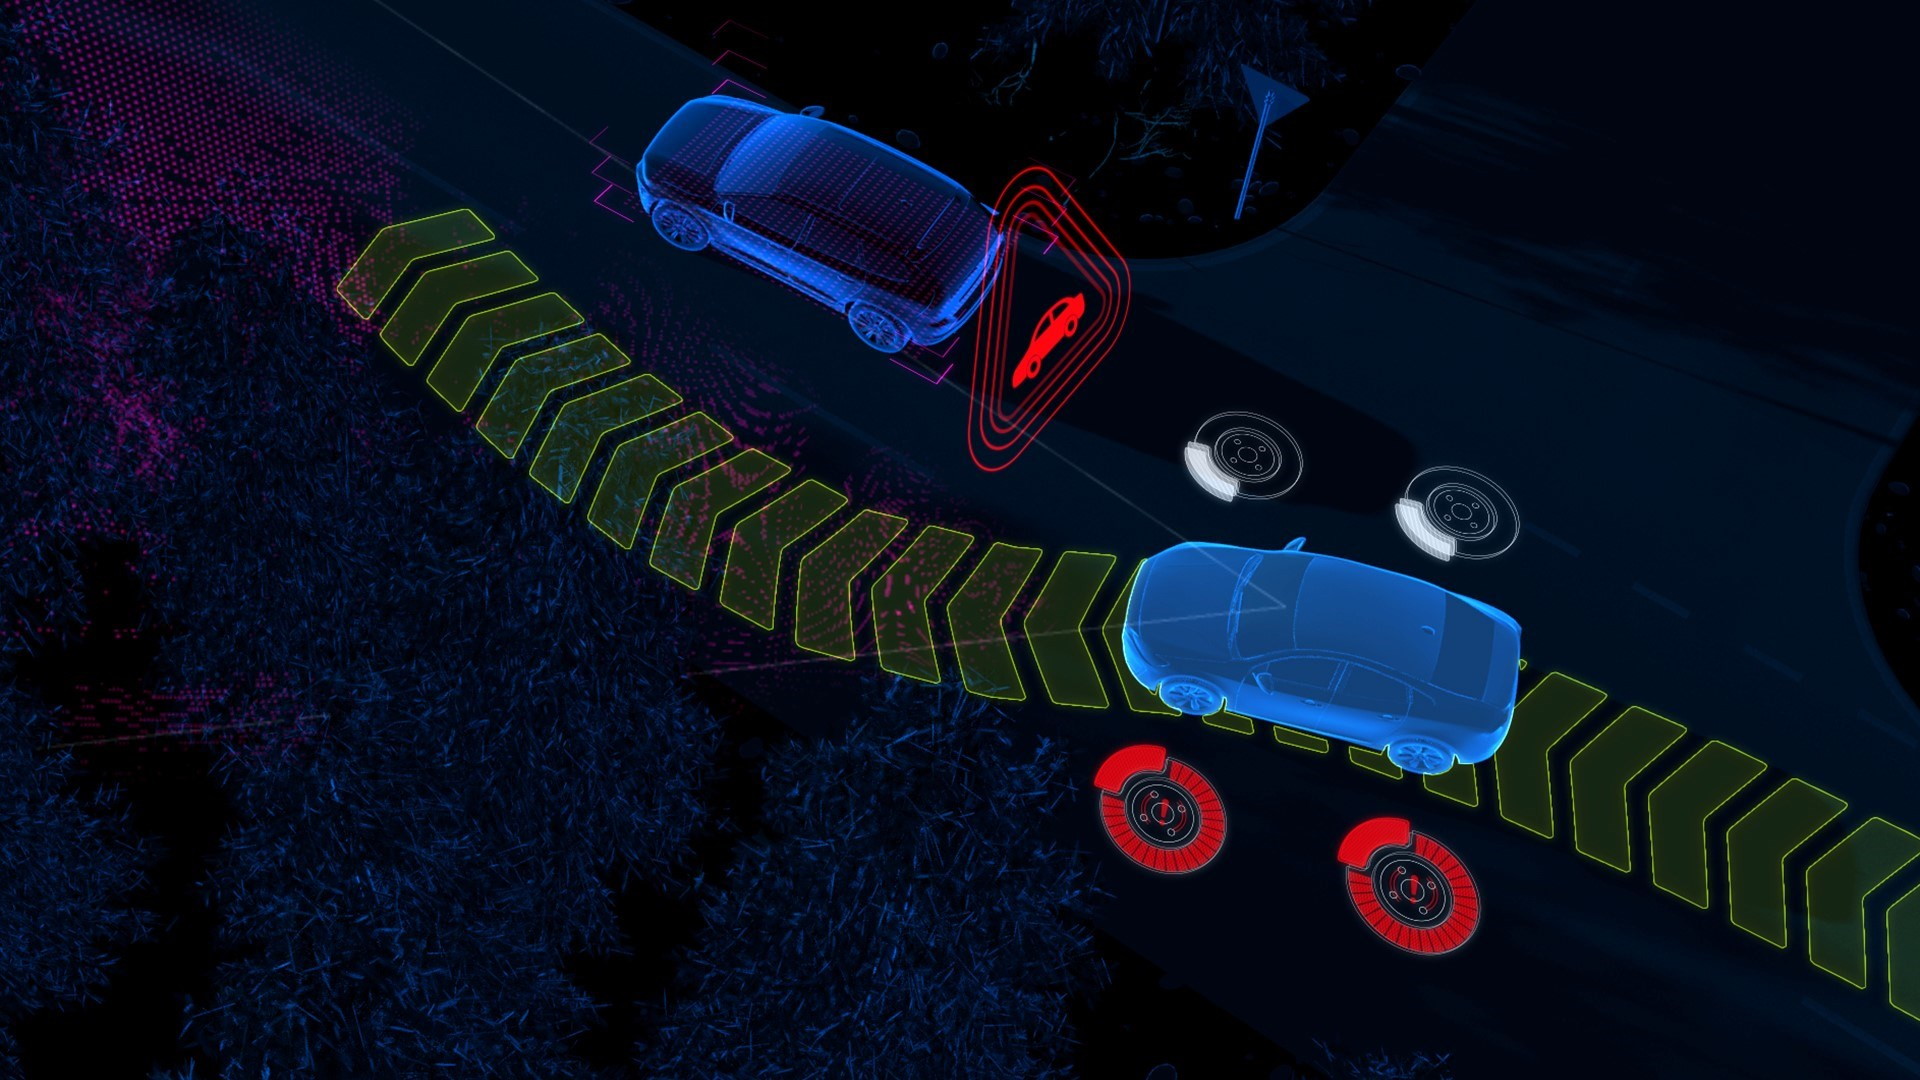
\includegraphics[width=.9\textwidth]{images/vhc1.JPG}
		\caption{}
		\label{fig:miror}
	\end{subfigure}\hfill%
	\begin{subfigure}{.48\textwidth}
		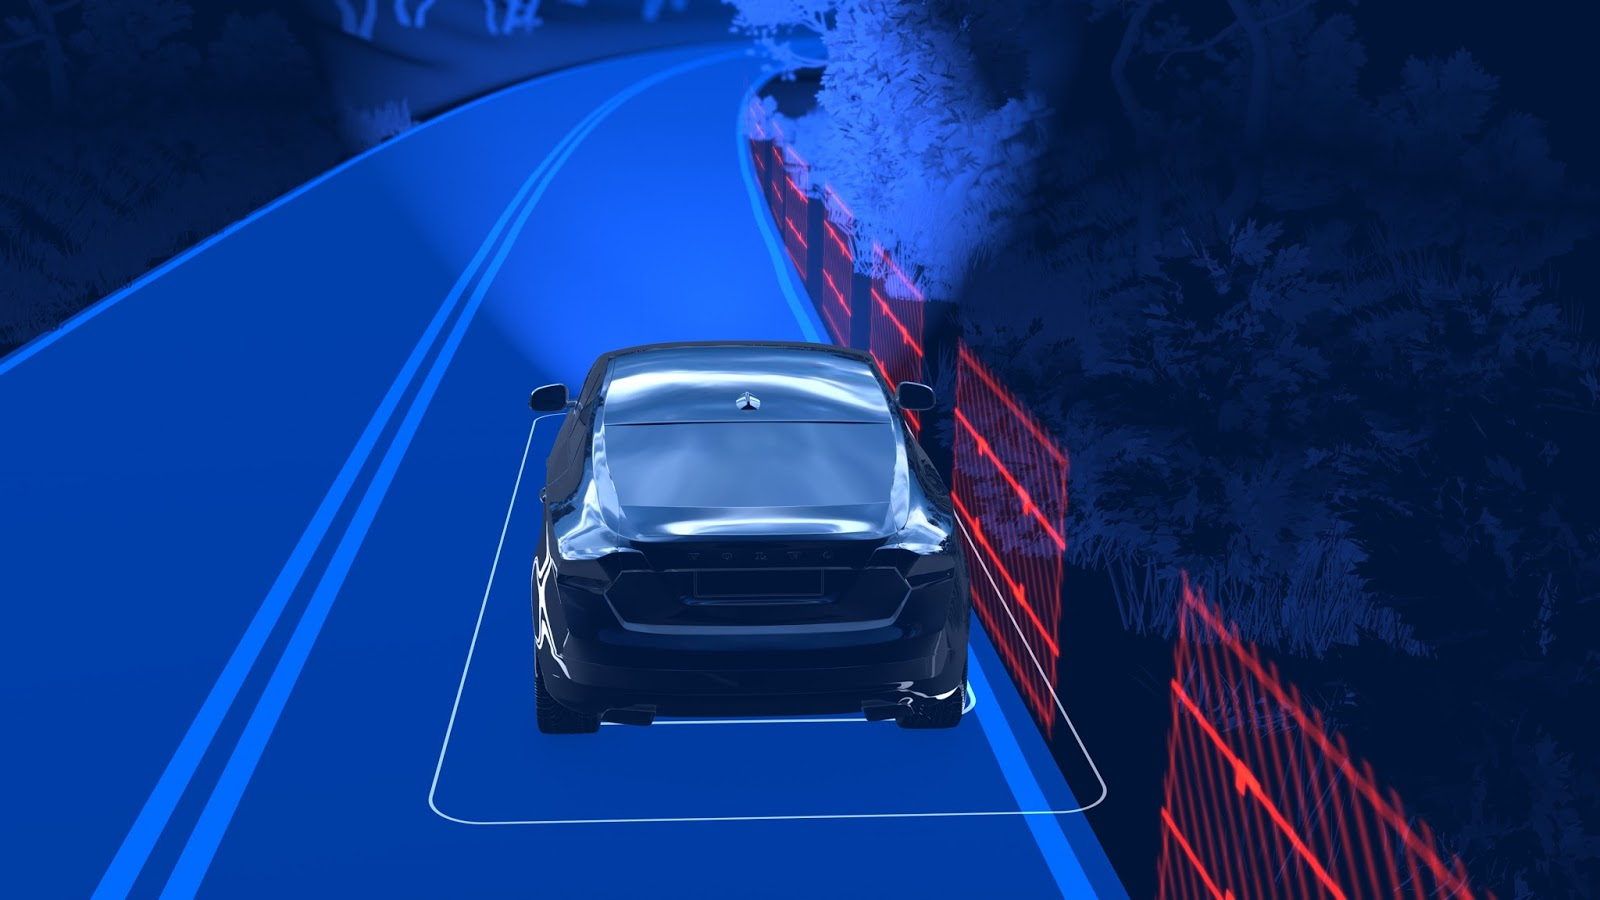
\includegraphics[width=.9\textwidth]{images/vhc2.jpg}
		\caption{}
		\label{fig:miror-couleur}
	\end{subfigure}
	\begin{subfigure}{.48\textwidth}
		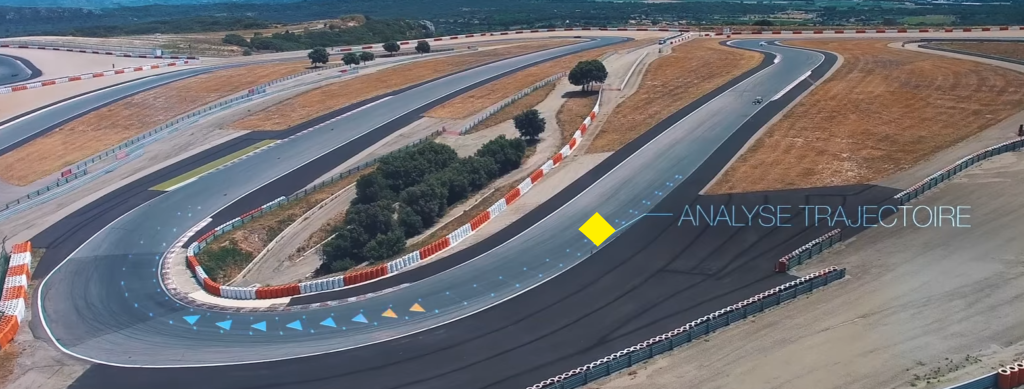
\includegraphics[width=.9\textwidth]{images/trajectoir.png}
		\caption{}
		\label{fig:miror-couleur}
	\end{subfigure}
	\caption{Analyse de trajectoire d'un véhicule autonome}
\end{figure}




 La deuxième hypothèse focalise sur l’endroit qui nous intéresse voire ou le positionnement de  véhicule dans un certain ensemble, où on peut supposé l’ensemble(la propriété) qui s’écrit sous la forme suivante:

%\edef\forall#1{\mathchar\number\forall{(#1)}\noexpand\;}

\begin{equation}
 \forall \; k \in \mathbb{N}, \;\;   x_{k} \in \{ x \in \reels^{d} / x^{T} Q x \ll \alpha  \}
 \end{equation}  
 Où $Q$ est symétrique définie positive et $\alpha \in \reels\cup \{+ \infty\}$ \\

alors l’équation 
$x^{T} Q x = ax^{2}+2bxy + cy^{2} =1$  représente une ellipse dont les axes pointent dans la direction des vecteurs propres et dont les longueurs sont $1 / \sqrt[]{\lambda_{1}},  1/ \sqrt[]{\lambda_{2}}$.
\textbf{Note}: Pour calculer une ellipse, on doit calculer le grand axe, le petit axe ça correspond au valeur propre de $Q$.


\subParagraphe{Le problème posé}
L’idée c’est de montrer finalement pour tout $x$, pour tout $k$:
\begin{itemize}
    \itemperso{} A-t-on un aperçu sur le nombre de points qui sont demandés? Le véhicule autonome va t-il s’arrêter?.
    \itemperso{} Pour faire la vérification sur le dépassement de capacité, a-t-on de variables bornées(après le calcule de la borne des $x_k$)?.
\end{itemize}

Faire preuve de sûreté, aussi preuve d’évitement face à un danger dans n'importe quelles conditions, sur n'importe quelle route. 



\section{Pr\'esentation du sujet}

\subsection{Formulation du problème}
Les travaux de recherche pr\'esent\'es dans ce m\'emoire se focalisent principalement sur un probl\`eme d’optimisation qu'on veut r\'esoudre et calculer d’une mani\`ere exacte (sans pour autant utiliser une sur-approximation).\\


 Effectivement on a $ \forall \; k  \in \mathbb{N}$, $\forall \; x \in X^{in}$ et à partir de (1.2)  
\begin{equation} 
  x^{T}A^{kT} Q A^{k}x \ll \alpha? \iff \underset{k \in \mathbb{N}}{\sup} \; \underset{x \in X^{in}}{\sup} x^{T} A^{kT} Q A^{k} x \ll \alpha?  
\end{equation} 
On peut toujours trouver $\gamma$ tel que 

\begin{equation}
\underset{k \in \mathbb{N}}{\sup} \; \underset{x \in X^{in}}{\sup} x^{T} A^{kT} Q A^{k} x \ll \gamma
\end{equation}
avec $\gamma$ est calcul\'e par un probl\`eme d'optimisation semi-d\'efinie.


Cependant, ce probl\`eme n\'ecessite un nombre infini de calculs et cela veut dire pour tout $k \in \mathbb{N}$, nous devons r\'esoudre exactement un probl\`eme qui est NP-difficile, et pour pouvoir le r\'esoudre, il suffit de discr\'etiser finement le probl\`eme pour $X^{in}$, ainsi pour $k \in \mathbb{N}$.

\subsection{Discr\'etisation du probl\`eme}

\subParagraphe{ Les besoins et les contraintes }
\vskip .5cm

Apr\`es le calcule de (1.2) par calcul it\'eratif, supposons maintenant $Q \succeq 0$ (car si on prend $Q \succ 0$, la limite tend vers l'infini et $ \{A^{k}x, k \in \mathbb{N}\}$ sera bornée), le probl\`eme est de calculer $K$ tel que: 

\begin{equation}
\underset{k \in \mathbb{N}}{\sup} \; \underset{x \in X^{in}}{\sup} x^{T} A^{kT} Q A^{k} x = \underset{k \in [K]}{\sup} \; \underset{x \in X^{in}}{\sup} x^{T} A^{kT} Q A^{k} x
\end{equation} 

Aussi, comme 

\begin{equation}
 \underset{x \in X^{in}}{\sup} x^{T} A^{kT} Q A^{k} x = \underset{x \in \mathcal{E} (X^{in})}{\sup} x^{T} A^{kT} Q A^{k} x
\end{equation} 

Alors, si $Q \succeq 0$ cela veut dire que $x \in \mathcal{E} (X^{in})$ fini car $X^{in}$ est un polytope, aussi d'apr\`es le lemme ci-dessous sur la notion de \textit{point extrémal},  bien entendu quand on maximise une fonction convexe sur un convexe compacte (polytope), c'est \'equivalent a maximiser cette fonction uniquement sur les points extr\'emaux. \\

$\lemme$  \textit{soit  $f: \reels^{d} \to \reels$ est convexe et continue sur un ensemble compact $U$ dans un espace de dimension finie $L$. Il résulte que
 $$\underset{x \in U} {\sup} \;f(x) \leq \underset{x \in \mathcal{E}(U)} {\sup} \; f(x)$$
où $\mathcal{E}(U)$ est l'ensemble des points extrêmes de $U$.} \\


De l'autre coté, comme $A^{k}$ tends vers la matrice nulle en l'infini, c'est équivalent à dire le rayon spectral de la matrice $A$ est strictement inférieur à 1.







\subsection{Normes matricielles}
Nous pouvons aussi définir des normes pour les matrices (carrées).

$\definition   $   \textit{Outre les trois propriétés requises pour la norme de matrice, certaines satisfont également à cette propriété supplémentaire non requise par toutes les normes de matrice.\\
La sous-multiplication: quelles que soient les matrices $A$ et $B$ on a: \;$\norm {AB} \leq \norm {A} \cdot \norm{B}$.
Pour toute norme dans $\reels^{d}$, la norme matricielle d'une matrice est $\norm{A} =\underset{x \in \reels^{d}\backslash 0 } \sup \frac{\norm{Ax}}{\norm{x}} $.}











\subsection{Quotient de Rayleigh}

Les (in)stabilités des systèmes dynamiques est l'un des problèmes de valeur propre qui sont omniprésents, et le quotient de rayleigh a pour but d'obtenir des estimations sur ces valeurs propres de plus en plus précises.


$\definition$ \textit{Le quotient de Rayleigh d'un problème de valeur propre généralisé $Ax = \lambda Bx$ est défini comme 
$$ RQ(x)= \frac{x^{T}Ax}{x^{T}Bx}$$
 où $A \succeq 0$ et $B \succ 0$.}

\textit{On peut voir que si $x$ est un vecteur propre telque $x \in \reels^{d} \backslash \{0\}$, $RQ (x)$ est la valeur propre correspondante avec $ \lambda_{min} \leq RQ(x) \leq \lambda_{max}$ où $\lambda_{min}$ et $\lambda_{max}$ sont les valeurs propres extrêmes de A.}

 
\textit{La premi\`ere classe de probl\`emes de valeurs propres est celle pour l'aquelle B est également défini positif.Un tel problème de valeur propre est équivalent \`a un probl\`eme de valeur propre symétrique $B^{-1 / 2}AB^{-1/2}y=\lambda x$ \cite{Ren-Cang}.}









\subsection{Élaboration de k}

\subParagraphe{ Appel de fonction de Lyapunov}
\vskip .5cm
En fait rayon spectrale de la matrice $A$ $<1$ équivaut a l'existence d 'une norme matricielle telle que $\norm{A} < 1$. Le fait que $A$ est une norme matricielle on a aussi $\norm{A^{k}} \leq \norm{A}^{k}$ qui tend vers 0.
% * <assale.adje@gmail.com> 2018-07-27T11:48:45.979Z:
% 
% "et donc norm(A^k)<norm(A)^k" doit etre placée dans une phrase à part. Ce n'est pas une conséquence de norm(A)<1 mais juste du fait que c'est un norme matricielle. 
% 
% ^.
 
 Soit $P \succ 0$ et $P-A^{T}PA \succ 0$.
 Comme $\norm{x}_{p} = \sqrt{x^{T}Px}$ définit une norme sur $\reels^{d}$
 alors
 \begin{equation}
  \norm{A}^{2}_{p} = \underset{x \in \reels^{d} \backslash {0} } \sup \frac{\norm{Ax}^{2}_{p}}{\norm{x}^{2}_{p} } =\underset{x \in \reels^{d} \backslash {0} } \sup \frac{x^{T}A^{T}PAx}{x^{T}Px}.
 \end{equation}
 sera la matrice norme.
 
 
  On définit pour $P\succeq 0$, $M= \underset{x \in \mathcal{E}(X^{in})}\sup x^{T}Px$, $L= \underset{x \in \mathcal{E}(X^{in})}\sup x^{T}Qx$

 \vskip .6cm
 
 $ \textbf{Proposition} $ \; \; \; \textit{$ L \lambda_{max}(Q)  \lambda_{min}(P)^{-1} M^{-1}$  et $0 < \norm{A}_p < 1$ } 
 \vskip .6cm
 
 $ \textbf{Preuve} $ \; \; \; \textit{pour les matrices symétriques $B, C$:}
 \vskip .2cm
  \textit{$  \; \; \;  \lambda_{k}(B)+ \lambda_{min}(C) \leq \lambda_{k}(B+C) \leq \lambda_{k}(B)+\lambda_{max}(C) $ et  $\rho(A)\leq \norm{A}_p$} \textit{d'après les Inégalités de Weyls }
 
 




\vskip .2cm
\subParagraphe{ La norme $\norm{A}_{p}$}
 \begin{equation}
\begin{array}{rrcl}
  & \norm{A}^{2}_{p}  & = &  \underset{x \in \reels^{d} \backslash {0} } \sup \frac{x^{T}A^{T}PAx}{x^{T}Px}    \\
  
     &  &  = &  \inf \{ t \geq 0 \; / \; \frac{x^{T}A^{T}PAx}{x^{T}Px} \leq t , \forall x \neq 0 \} \\
     
       &  &  = &   \inf \{ t \geq 0 \; / \; tx^{T}Px \geq x^{T}A^{T}PAx , \forall x \neq 0 \}   \\
       
         &  &  = &   \inf \{ t \geq 0 \; / \;  x^{T} (tP-A^{T}PA)x \geq  0, \forall x \neq 0 \}     \\
         
          &  &  = &   \inf \{ t \geq 0 \; / \;  tP-A^{T}PA \geq 0 \} \; < 1     \\
                   
\end{array}
\end{equation}

Ensuite
\begin{equation}
\left \{ \begin{array}{rrcl}
\min  & \lambda_{max} (P) & & \\
      & P-A^{T}PA-\varepsilon Id & \succeq & 0 \\
      & P                   & \succ & 0 \\
\end{array} \right.
\end{equation}

Tel que le PO a suggéré de résoudre le SDP en utilisant CSDP est le suivant  

\begin{equation}
  \left \{ \begin{array}{rrcl}
 \min  &  t & & \\
 & tId-P & \succeq & 0 \\

      & P-A^{T}PA-\varepsilon Id & \succeq & 0 \\
      & P                   & \succ & 0 \\
\end{array} \right.
\end{equation}


\vskip .5cm
\subParagraphe{Version1}

\vskip .5cm
Soit $P$ une solution discrète de Lyapunov et $k \in \mathbb{N}$, $x \in \mathcal{E}(X^{in})$.

\begin{equation}
\begin{array}{rrcl}
  & x^{T} A^{kT} Q A^{k} x   & \leq  &   \lambda_{max}(Q) \norm{A^{k}x }^{2}_{2}  \;\;\; \rightarrow \; Quotient\; de \; Rayleigh  \\
  
     &  &  \leq &  \lambda_{max}(Q) \norm{A^{k}x }^{2}_{p} \lambda_{min}(P)^{-1} \\
     
       &  &  \leq &  \lambda_{max} (Q) \lambda_{min}(P)^{-1} \norm{A^{k} }^{2}_{p}  \norm{x }^{2}_{p}  \;\;\; \rightarrow \; norme\; subordonnee   \\
       
         &  &  \leq &  \lambda_{max} (Q) \lambda_{min}(P)^{-1} \norm{A}^{2k}_{p}  M  \;\;\; \rightarrow \; norme\; matricielle    \\
           
\end{array}
\end{equation}


comme $\norm{A}^{2}_{p} < 1$ cela veut dire $\ln \norm{A}^{2}_{p} < 0$


On cherche $k$ tel que 

\begin{equation}
\begin{array}{rrcl}
  & \norm{A}^{2k}_{p} \lambda_{max}(Q)\lambda_{min}(P)^{-1} M  & \leq  &   L = \underset{x \in \mathcal{E}(X^{in})} \sup x^{T}Qx \\
  
     & \norm{A}^{2k}_{p} &  \leq & L  \lambda_{min}(P)  \lambda_{max}(Q)^{-1} M^{-1} \\
     
   
       
         & k \ln \norm{A}^{2}_{p} &  \leq &  \ln (L \lambda_{min}(P) \lambda_{max}(Q)^{-1} M^{-1})    \\
         
         
             & K &  \geq & E \Big ( \frac{ \ln (L \lambda_{min}(P) \lambda_{max}(Q)^{-1} M^{-1})}{\ln \norm{A}^{2}_{p}} \Big ) +1\\
           
\end{array}
\end{equation}

\newpage
\subParagraphe{Version2}

\vskip .5cm
On cherche une fonction $P$ telle que 

\begin{equation}
  \left \{ \begin{array}{rrcl}
 \min  &  \lambda_{\max}(P) & & \\
 & \lambda_{\max}(Q)P-Q & \succeq & 0 \\

      & P-A^{T}PA & \succeq & 0 \\
      & P                   & \succ & 0 \\
\end{array} \right.
\end{equation}

\begin{equation}
\begin{array}{rrcl}
  & x^{T} A^{kT} Q A^{k} x   & \leq  &   \lambda_{max}(Q)\;\; x^{T} A^{kT} P A^{k} x \\
  
     &  &  \leq &  \lambda_{max}(Q) \norm{A^{k}x }^{2}_{p} \\
         
    
                & k &  \geq & E \Big ( \frac{ \ln (L \lambda_{max}(Q)^{-1} M^{-1})}{\ln \norm{A}^{2}_{p}} \Big ) +1\\
         
                 & K_{1} &  \geq & E \Big ( \frac{ \ln (L \lambda_{max}(P^{-1/2}QP^{-1/2})^{-1} M^{-1})}{\ln \norm{A}^{2}_{p}}\Big ) +1  \;\;\; \rightarrow \;En \; utilisant \; le \;Quotient\; de \; Rayleigh \\        
         
         
         
\end{array}
\end{equation}











\section{Liste de progiciels int\'egr\'es}

\subsection{CSDP, C Library for Semidefinite Programming}
\subsubsection{Définition}

Un probl\`eme d\'optimisation convexe avec des in\'egalit\'es matricielles lin\'eaires peut \^etre r\'esolu tr\`es efficacement par programmation semi-d\'efinie.Dans cette recherche , le probl\`eme d\'optimisation est r\'esolu avec la biblioth\`eque C CSDP (C Library for semidefinite programming)\cite{Borchers.B:}.CSDP est \'ecrit en $C$ pour l\'efficacit\'e et la portabilit\'e.\\

CSDP comporte \'egalement un certain nombre de caract\'eristiques qui la rendent tr\`es flexible.CSDP peut travailler avec des matrices sym\'etriques g\'en\'erales ou avec des matrices qui ont une structure diagonale de bloc d\'efinie.Cette biblioth\`eque contient \'egalement des routines pour lire et \'ecrire des probl\`emes SDP et des solutions \`a partir de fichiers.Un programme de r\'esolution autonome est inclus pour r\'esoudre les probl\`emes SDP qui ont \'et\'e \'ecrits dans le format sparse SDPA\cite{SDPA}.

\subsubsection{Le probl\`eme SDP}
CSDP résout les problèmes de programmation semi-définie sous forme:

\begin{equation}
\begin{array}{rrcl}
\max  & \mbox{tr}\; (CX) & & \\
      & A(X) & = & b \\
      & X                   & \succeq & 0 \\
\end{array}
\end{equation}

avec $A_{i}= \mbox{tr}(A_{i}X)$ où $X \succeq 0$ signifie que $X$ est semi-défini positif, $C$ et tous $A_{i}$ sont des matrices symétriques de même taille et $b$ est un vecteur de longueur $m$.\\

Le dual de ce SDP est:

\begin{equation}
\begin{array}{rrcl}
\min  & a^{T}y  & & \\
      & A^{T}(y)-C & = & Z \\
      & Z                   & \succeq & 0 \\
\end{array}
\end{equation}
où
\begin{equation}
A^{T}(y)=\sum_{i=1}^{m} y_{i}A_{i}.
\end{equation}

Et les matrices $C$, $X$ et $Z$ sont traitées comme des matrices diagonales.

\subsubsection{SDP en forme standard}
Considérons, par exemple, le programme semi-défini proposé par le professeur Borchers \cite{Borchers.B:}.Soit le PO a suggéré de résoudre le SDP:

\begin{equation}
\begin{array}{rrcl}
\min  & 0 &&  \\ 
&P - A^{T}PA - \varepsilon I & \succeq & 0 \\ 
&P &\succ & 0\\ 
\end{array}
\end{equation}
% * <assale.adje@gmail.com> 2018-07-27T11:56:27.436Z:
% 
% Ou est passée la valeur propre maximale de P?
% 
% ^.

où $\varepsilon$ est une petite constante positive(nous utiliserons $\varepsilon = 0.01$ dans la suite.) comme $A^{T}P A$ est semi-défini positif et que $\varepsilon I$ est défini positif, ces contraintes imposent $P \succ 0$ (En fait, $P \succeq \varepsilon I $, donc la plus petite valeur propre de $P$ sera supérieur ou égal à $\varepsilon $.) \\

La modélisation de paquets (Packages) comme CVX et Yalmip peuvent facilement transformer cette formulation en un SDP qui peut être résolu par une variété de solveurs tels que SDPT3, SeDuMi, CSDP, SDPA,.. etc.Cependant, le PO veut voir comment transformer cela en une forme standard SDP \cite{Borchers.B:}.



\begin{equation}
\begin{array}{rrcl}
\max  & \mbox{tr}\; (CX)  & & \\
     &\mbox{tr}\;(A_{i}X)&=&b_{i}\;\; i=1, 2, \ldots, m \\
      & X       & \succeq & 0 \\
     
\end{array}
\end{equation}

La première étape consiste à introduire une variable lâche $S$ et à écrire le problème comme  
\begin{equation}
\begin{array}{rrcl}
\max  & 0  & & \\
     & P- A^{T} PA - S &=& \varepsilon I \\
      & S       & \succeq & 0 \\
       & P       & \succeq & 0 \\
\end{array}
\end{equation}

 La contrainte $P- A^{T} PA - S = \varepsilon I$ est linéaire dans les éléments de $P$, bien que cela ne soit pas immédiatement évident.L’observation clé est que  

 \begin{equation}
 A^{T}PA=\underset{ j,k } \sum P_{j,k} \; \underset{i,l} \sum A_{j,i}A_{k,l} E_{i,l}
 \end{equation}  
 
 Par la suite 
 
  \begin{equation}
P- A^{T}PA=\underset{ j,k } \sum P_{j,k} \Big( E_{j,k}- \underset{i,l} \sum A_{j,i}A_{k,l} E_{i,l} \Big)
 \end{equation}  
 
 Et enfin 
 
 
   \begin{equation}
P- A^{T}PA-\varepsilon I=\underset{ j,k } \sum P_{j,k} \underbrace{\Big( E_{j,k}- \underset{i,l} \sum A_{j,i}A_{k,l} E_{i,l} \Big)}_{A_{i}} -\underbrace{\varepsilon I}_{A_{0}} 
 \end{equation}  
% * <assale.adje@gmail.com> 2018-07-27T11:56:58.620Z:
% 
% Il faut terminer le travail en écrivant explicitement le dual à partir de ce LMI.
% 
% ^.
 
 \subParagraphe{Exemple d'application}
 
 \vspace*{.5cm}
 
 Supposons que le PO a une matrice $A$ de taille $(2\times2)$ 
 
 \begin{equation}
A=\left[
\begin{array}{rrrrrrr}
 A_{1,1} & A_{1,2}    \\ 
 A_{2,1} & A_{2,2}   \\ 
    
\end{array}
\right]
\end{equation}


Et pour trouver une matrice symétrique $P$, nous avons besoin de 3 contraintes d'égalité linéaire pour les éléments (1,1), (1,2), (2,2) de l'égalité matricielle 

 \begin{equation}
 \begin{array}{rrcl}
 
&P_{1,1} \left[ E_{1,1} - \left( A_{1,1} A_{1,1} E_{1,1}+ A_{1,1} A_{1,2} E_{1,2}+A_{2,1} A_{1,1} E_{2,1} +A_{1,2} A_{1,2} E_{2,2}       \right) \right] &=&\varepsilon \\

&P_{1,2} \left[ E_{1,2} - \left( A_{1,1} A_{2,1} E_{1,1}+ A_{1,1} A_{2,2} E_{1,2}+A_{1,2} A_{2,1} E_{2,1} +A_{1,2} A_{2,2} E_{2,2}       \right) \right] &=&\varepsilon \\

&P_{2,2} \left[ E_{2,2} - \left( A_{2,1} A_{2,1} E_{1,1}+A_{2,1} A_{2,2} E_{1,2} +A_{2,2} A_{2,1} E_{2,1} + A_{2,2} A_{2,2} E_{2,2}      \right) \right] &=&\varepsilon \\

\end{array}
 \end{equation}
 
 Ensuite
 
   \begin{equation}
 \begin{array}{rrcl}
 
&E_{1,1} \left[ P_{1,1} \left(1-  A_{1,1} A_{1,1}\right)- P_{1,2} \left(  A_{1,1} A_{2,1}\right) -P_{2,1} \left( A_{2,1} A_{1,1}\right) -P_{2,2} \left(A_{2,1} A_{2,1}\right)       \right]-S_{1,1} &=&\varepsilon \\

&E_{1,2} \left[ P_{1,1} \left( A_{1,1} A_{1,2}\right)+ P_{1,2} \left( 1- A_{1,1} A_{2,2}\right) -P_{2,1} \left( A_{2,1} A_{1,2}\right) -P_{2,2} \left( A_{2,1} A_{2,2}\right)       \right]-S_{1,2} &=&\varepsilon \\


&E_{2,2} \left[ P_{1,1} \left( A_{1,2} A_{1,2}\right)- P_{1,2} \left(  A_{1,2} A_{2,2}\right) -P_{2,1} \left( A_{2,2} A_{2,1}\right) +P_{2,2} \left(1-  A_{2,2} A_{2,2}\right)       \right]-S_{2,2} &=&\varepsilon \\


\end{array}
 \end{equation}
 
 
  Enfin nous intégrons $P$ et $S$ dans une matrice diagonale par bloc 
 
 \begin{equation}
X=\left[
\begin{array}{cc}
P &  0\\
0&  S \\
\end{array}
\right]
\end{equation}

Le problème devient
 
 \begin{equation}
\begin{array}{rrcl}
\max  & \mbox{tr}\; (CX)  & & \\
     &\mbox{tr}\;(A_{1}X)&=& \varepsilon \\
     &\mbox{tr}\;(A_{2}X)&=&\varepsilon \\
     &\mbox{tr}\;(A_{3}X)&=& \varepsilon \\
      & X       & \succeq & 0 \\
     
\end{array}
\end{equation}

où 

\begin{equation}
C=0
\end{equation}

\begin{equation}
A_{1}=\left[
\begin{array}{cccc}
1-  A_{1,1} A_{1,1}  &- A_{1,1} A_{2,1} & 0 & 0 \\
- & -A_{2,1} A_{2,1} & 0 & 0 \\
0    &   0  & -1.0 & 0 \\
0    &   0  &  0   & 0 \\
\end{array}
\right]
\end{equation}


\begin{equation}
A_{2}=\left[
\begin{array}{cccc}
-A_{1,1} A_{1,2}& 1- A_{1,1} A_{2,2} & 0 & 0 \\
- & -A_{2,1} A_{2,2} & 0 & 0 \\
0    &   0  &  0 & -1.0 \\
0    &   0  &  0   & 0 \\
\end{array}
\right]
\end{equation}

\begin{equation}
A_{3}=\left[
\begin{array}{cccc}
-A_{1,2} A_{1,2} & - A_{1,2} A_{2,2} & 0 & 0 \\
- & 1-  A_{2,2} A_{2,2} & 0 & 0 \\
0    &   0  &  0 & 0 \\
0    &   0  &  0  & -1.0 \\
\end{array}
\right]
\end{equation}
Prenons l'exemple d'une matrice carrée
 \begin{equation}
A=\left[
\begin{array}{rrrrrrr}
 0.5 & -0.4    \\ 
 1 & -0.5   \\ 
    
\end{array}
\right]
\end{equation}
Après avoir passer par le calcul (2.12) et d'écrire le résultat obtenu sous forme matrice diagonale par bloc, le problème s'écrit au format SDPA comme suit


\begin{lstlisting}
3
2
2 2
0.01 0.01 0.01
1 1 1 1 0.75
1 1 1 2 -0.5
1 1 2 2 -1.0
1 2 1 1 -1.0
2 1 1 1 0.2
2 1 1 2 1.25
2 1 2 2 0.5
2 2 1 2 -1.0
3 1 1 1 -0.16
3 1 1 2 -0.2
3 1 2 2 +0.75
3 2 2 2 -1.0
\end{lstlisting}

Après la résolution de ce problème en utilisant CSDP, on obtient:
\begin{equation}
P=\left[
\begin{array}{cc}
  P_{1,1}   & P_{1,2}\\
 P_{2,1}   & P_{2,2} \\
\end{array}
\right]
=\left[
\begin{array}{cc}
  40.36   & -9.27\\
 -9.27  & 24.39 \\
\end{array}
\right]
\end{equation}

\begin{equation}
S=\left[
\begin{array}{cc}
   S_{1,1}   &   S_{1,2}  \\
S_{2,1}    &  S_{2,2}  \\
\end{array}
\right]
=\left[
\begin{array}{cc}
15.14  & -1.46\\
-1.46   & 15.54 \\
\end{array}
\right]
\end{equation}


Il est facile de vérifier que $P$ possède toutes les propriétés requises.\\
Il y a une infinité de solutions à ce problème il n’y a aucune raison de s’attendre à ce que tous les solveurs renvoient la même solution.\\
On peut également ajuster la fonction objectif ou ajouter des contraintes supplémentaires pour pousser la solution dans une direction souhaitée. Par exemple, on peut vouloir minimiser la valeur propre maximale de $P$ ou minimiser la somme des valeurs propres de $P$.
% * <assale.adje@gmail.com> 2018-07-27T11:59:14.502Z:
% 
% Il faut dire que d'office SDP minimise la valeur propre maximale
% 
% ^.

 \subsubsection{L'interface CSDP}
 
 
 
 









\begin{itemize}
	\itemperso{Trouver une solution initial}
	
	La bibliothèque CSDP contient une routine qui permet d’allouer tout le stockage requis pour trouver une solution initiale. La séquence d’appel pour cette routine est:
                         $$ initsoln(n,k,C,a,constraints,pX0,py0,pZ0).$$
	\itemperso{Appel de la routine SDP}
	
	 C’est une version facile à appeler de la routine sdp.Il prend en entrée un problème sous la forme $$(n, k, C, a, constraints, constant\_offset)$$ et une solution initiale ($X$, $y$, $Z$), allouer l’espace de stockage ensuite faire l’appel à {\tt sdp()} pour résoudre le problème.La solution est retournée dans $X$, $y$, $Z$, {\tt pobj} , {\tt dobj}, et le code de retour de sdp est retourné comme valeur de retour de  {\tt easy\_sdp} (voir 3.1.5).
	
\end{itemize}


\subsubsection{Lecture et écriture de données}

Fonctions pour lire et écrire des données de programme semi-définies et des solutions au format SDPA.


\begin{itemize}
    \itemperso{Usage}
    
read\_prob(fname,pn,pk,pC,pa,pconstraints,printlevel)\\
write\_prob(fname,n,k,C,a,constraints)\\
read\_sol(fname,n,k,C,pX,py,pZ)\\
write\_sol(fname,n,k,X,y,Z)

    
    
    \itemperso{Arguments}
    \begin{itemize}
        \subitemperso{fname} Le nom du fichier à lire ou à écrire.
        \subitemperso{n, pn} La dimension de $X$.
        \subitemperso{k, pk}  Nombre de contraintes.
        \subitemperso{C, pC} La matrice $C$.
        \subitemperso{a, pa} Le vecteur $a$.
        \subitemperso{X, pX} La solution primal $X$.
        \subitemperso{Z, pZ } La matrice dual $Z$.
        \subitemperso{ y,  py} Le vecteur dual $y$.
        \subitemperso{printlevel} $= 0$ pour aucune sortie, $= 1$ pour la normale
                      sortie,$\succ 1$ pour le débogage.
        \subitemperso{ constraints, pconstraints} Les contraintes. 
                      
                      
                      
        
        
    \end{itemize}
    
    \itemperso{Détails}
    
    Les matrices structurées par blocs doivent être spécifiées comme décrit dans\cite{Borchers.B:}.Les fichiers lus doivent être au format SDPA\cite{SDPA}.Cependant, ces fonctions ne prennent pas en charge les commentaires ou les caractères de regroupement par exemple (les accolades, les parenthèses) dans la spécification des tailles de bloc.
    
    \itemperso{Valeurs}
    
    La routine {\tt read\_prob} alloue tout le stockage requis par le problème d’un coté, de l’autre coté {\tt write\_sol}  renvoie 0 en cas de succès et se termine si elle est incapable d’écrire le fichier de solution. 
    
\end{itemize}

\subParagraphe{Spécificités}
\vskip .5cm
\begin{itemize}
    \itemperso{Arguments}
    \begin{itemize}
    \subitemperso{n}  Ce paramètre donne la dimension des matrices $X$, $C$ et $Z$. 
    \subitemperso{k}  Ce paramètre donne le nombre de contraintes.
    \subitemperso{C} Ce paramètre donne la matrice $C$ et définit implicitement la structure en blocs des matrices diagonales.
    \subitemperso{a} Ce paramètre donne le vecteur de droite $a$.
    \subitemperso{constraints} Ce paramètre spécifie les contraintes de problème.
    \subitemperso{constant offset} Ce scalaire est ajouté aux valeurs des objectifs primal et dual.
    
    \subitemperso{pX} En entrée, ce paramètre donne la solution initiale primal X.
    \subitemperso{py} En entrée, ce paramètre donne la solution initiale dual y.
    \subitemperso{pZ} En entrée, ce paramètre donne la solution initiale dual Z.
     \end{itemize}
    
    
    \itemperso{Valeurs}
    \begin{itemize}
        \subitemperso{pX}  En sortie, ce paramètre donne la solution optimale primal X. 
        \subitemperso{py}  En sortie, ce paramètre donne la solution optimale dual y.
        \subitemperso{pZ} En sortie, ce paramètre donne la solution optimale dual Z.
        \subitemperso{ ppobj} Valeur objective optimale primal.
        \subitemperso{pdobj} Valeur objective optimale dual.
    \end{itemize}
    
    \itemperso{Statut}
    
    Statut de la solution renvoyée\\
    \begin{tabular}{r l} 
  
 0 &{\tt Succès }. Problème résolu à une précision totale.  \\ 
 1 &{\tt Succès}. Le problème est irréalisable primal. \\ 
 2 &{\tt Succès}. Le problème est irréalisable dual. \\ 
 3 &{\tt Succès}. partiel. Solution trouvée mais la précision n’a pas été atteinte. \\ 
 4 &{\tt Échec }. Nombre maximal d’itérations atteint. \\ 
 5 &{\tt Échec }. Coincé à la limite de la faisabilité primal. \\  
 6 &{\tt Échec}. Stuc au bord de l’infaisabilité dual. \\ 
 7 &{\tt  Échec}. Manque de progrès. \\ 
 8 &{\tt Échec}. $X$ ou $Z$ (ou Newton système O) est singulier. \\ 
 9 &{\tt Échec }. Valeurs NaN ou Inf détectées. \\ 
  
\end{tabular}
    
    \itemperso{Entrées du programme final}
    \vskip .5cm
    \begin{lstlisting}[language=C++]
#include <stdlib.h>
#include <stdio.h>

/*
 * Include CSDP declarations so that we'll know the calling interfaces.
 */

#include "../include/declarations.h"

/*
 * The main program.  Setup data structures with the problem data, write
 * the problem out in SDPA sparse format, and then solve the problem.
 */
 int main()
{
  /*
   * The problem and solution data.
   */

  struct blockmatrix C;
  double *b;
  struct constraintmatrix *constraints;

  /*
   * Storage for the initial and final solutions.
   */

  struct blockmatrix X,Z;
  double *y;
  double pobj,dobj;

  /*
   * blockptr will be used to point to blocks in constraint matrices.
   */

  struct sparseblock *blockptr;

  /*
   * A return code for the call to easy_sdp().
   */

  int ret,pn,pk;

  /*
   * Write the problem out in SDPA sparse format.
   */

 read_prob("version_final.dat",&pn,&pk,&C,&b,&constraints,0.0);
 write_prob("version_final.dat-s",4,3,C,b,constraints);

  /*
   * Create an initial solution.  This allocates space for X, y, and Z,
   * and sets initial values.
   */

  initsoln(4,3,C,b,constraints,&X,&y,&Z);

  /*
   * Solve the problem.
   */

  ret=easy_sdp(4,3,C,b,constraints,0.0,&X,&y,&Z,&pobj,&dobj);
  if (ret == 0)
    printf("The objective value is %.7e \n",    (dobj+pobj)/2);
  else
    printf("SDP failed.\n");

  /*
   * Write out the problem solution.
   */

  write_sol("version_final.sol",4,3,X,y,Z);

  /*
   * Free storage allocated for the problem and return.
   */

  free_prob(4,3,C,b,constraints,X,y,Z);
  exit(0);
  
}
\end{lstlisting}

 \newpage
 \itemperso{Sortie du programme final}
 \vskip .4cm
 \begin{figure}[ht]
	\centering
	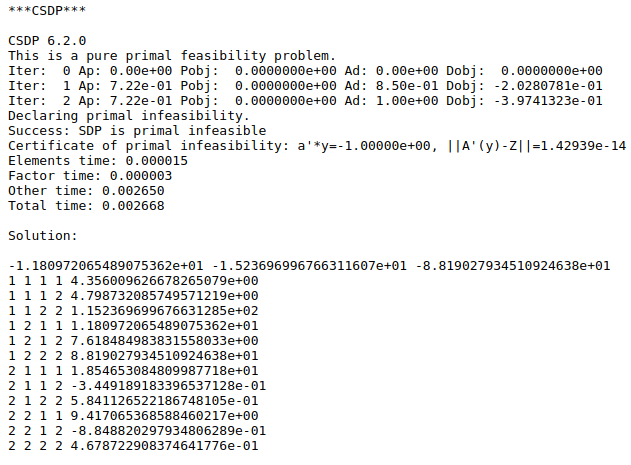
\includegraphics[width=.6\textwidth]{images/output.png}
	\caption{Résultats obtenus après l'appel d'un solveur CSDP}
	\label{fig:CSDP Résult}
\end{figure}

 \end{itemize}
 
 
 
 





\subsection{C-Library cddlib pour l'énumération des Sommets}
\subsubsection{Définition}

La bibliothèque cddlib est une implémentation C de la méthode double description de Motzkin et al.Pour générer tous les sommets(c’est-à-dire les points extrêmes) et les rayons extrêmes d’un polyèdre convexe général dans $ \reels^{d}$ donnée par un système d’inégalités linéaires:  

\begin{equation}
     P= \{ x=({x}_{1}, \ldots, {x}_{d})^{T}  \;: \;Ax \leq b  \}     
\end{equation}

% * <assale.adje@gmail.com> 2018-07-27T11:59:59.141Z:
% 
% Attention la relation d'ordre n'est pas la même il ne faut plus utiliser le même signe d'inégalité
% 
% ^.
où $A$ est une matrice réelle $m$ x $d$ donnée, $b$ est un m-vecteur donné et 0 est le m-vecteur de tous les zéros.


\subsection{ H-representation \& V-polyhedron}

Un polyèdre peut être décrit par une liste d'inégalités (H-representation) ou par une liste de ses sommets + rayons extrêmes (V-representation ) où "+" est la somme de \textit{Minkowski}\footnote{(en géométrie) une opération sur les parties d'un espace vectoriel. À deux parties $A$ et $B$ elle associe leur ensemble somme, formé des sommes d'un élément de $A$ et d'un élément de $B$}. Cddlib\cite{cdd/cddplus} permet de convertir un programme qui représente un polyèdre par H-representation en son V-representation, et vice versa.Ces problèmes sont connus respectivement au niveau de l’énumération des sommets et des problèmes de \href{http://le-terrier-de-lapineige.over-blog.com/2014/09/bm-c-comme-convex-hull-un-outil-de-modelisation-polyvalent.html}{coque convexe}.
\newpage
\subsection{ formats de fichiers avec l'implémentation sur un exemple}
% * <assale.adje@gmail.com> 2018-07-27T12:02:53.141Z:
% 
% Copier-coller!!
% 
% ^.
L’entrée pour Cddlib est une H-représentation ou V-representation d’un polytope.Ces fichiers ont les formats suivants:
 \begin{figure}[ht]
	\centering
	\begin{subfigure}{.20\textwidth}
		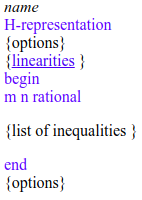
\includegraphics[width=\textwidth,scale=0.7]{images/H_representation.png}
		\caption{H-Représentation}
		\label{fig:h_represt}
	\end{subfigure}\hfill%
	\begin{subfigure}{.33\textwidth}
		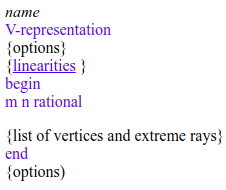
\includegraphics[width=\textwidth,scale=0.7]{images/V_representation.png}
		\caption{V-Représentation}
		\label{fig:v_represt}
	\end{subfigure}\hfill%
	\caption{H-Représentation \& V-Représentation}
	\end{figure}
    
    
    
    \subParagraphe{Représentation en demi-espace(H-representation) }
    
    \vspace*{.5cm}
    
La H-representation d'un polytope convexe $S$ n'est qu'un ensemble d'inégalités linéaires correspondant à l'intersection des demi-espaces: $$S = (x \; |\; Ax\leq b)$$
 Il est toujours possible de normaliser la représentation pour que les composantes de b soient 1 ou 0. Lorsque toutes ces composantes sont nulles, le polyèdre est un cône convexe polyédrique pointé à l'origine. Quand tous les composants de b sont des uns, rien ne peut être dit avec certitude Mais, à l'inverse, pour un polytope on a seulement un dans le vecteur colonne de son H-representation. Nous nous retrouvons donc avec le vocabulaire suivant:
 
 $$Polyedre: P=\{(x \; | \; Ax\leq b)\} $$
 $$Cone \; polyedrique: P=\{(x \; | \; Ax\leq 0)\}$$
$$Polytope: P=\{(x \; | \; Ax\leq 1)\}\\ $$

Prenons en exemple ces inégalités:
 \begin{equation}
      1+{x}_{1} \succeq 0 \;\;\; \;\;\;  1+{x}_{2}\succeq 0  \;\;\;\; \; \; 1-{x}_{1} \succeq 0 \;\; \;\; \;\;   1-{x}_{2} \succeq 0 
\end{equation}

ces inégalités sont entrées comme la ligne 
\begin{equation}
      {a}_{0} \; {a}_{1}, \ldots ,{a}_{n-1}    
\end{equation}

et qui serait représenté par le fichier d’entrée 


 \begin{figure}[ht]
	\centering
\fbox{	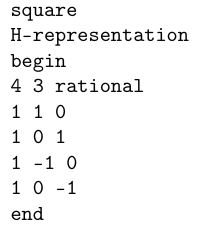
\includegraphics[width=.2\textwidth]{images/exempl-Hrepst.png}}
	\label{fig:ex_hreprest}
\end{figure}

\subParagraphe{Fichier V-representation}

\vspace*{.5cm}

La représentation de sommet (V-representation) d'un polyèdre le décrit en termes de points (sommets), comme il génère des vecteurs appelés rayons. Informellement, les sommets sont les limites "finies" du polyèdre, tandis que les rayons sont les "infinis". Un polytope n'a que des sommets, tandis qu'un cône polyédrique ne contient que des rayons. Formellement, les points x du polyèdre sont décrits par:
$$x=conv(V)+coni(R)$$

où $conv$ désigne la coque convexe d'un ensemble de sommets $V=\{ v_1,\ldots, v_p \}$

tandis que $coni$ est la coque conique d'un ensemble de rayons $R=\{ r_1,\ldots, v_q \}$


chaque sommet (voir Figure \ref{fig:v_represt}) est donnée sous la forme:
\begin{equation}
      1 \;{v}_{0} \; {v}_{1}, \ldots ,{v}_{n-1}    
\end{equation}

chaque rayon est donnée sous la forme 

\begin{equation}
      0 \;{r}_{0} \; {r}_{1}, \ldots ,{r}_{n-1}    
\end{equation}

où  $ 0 \;{r}_{0} \; {r}_{1}, \ldots ,{r}_{n-1}$ est un point sur le rayon.


Il doit y avoir au moins un sommet dans chaque fichier. Pour les polyèdres bornés, il n’y aura pas de rayons entrés.\\

Par exemple, l’entrée de fichier V-representation serait représenter comme suit: 

\begin{figure}[ht]
	\centering
\fbox{	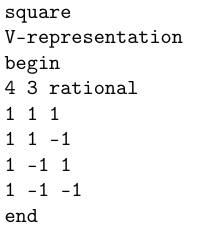
\includegraphics[width=.2\textwidth]{images/exem-Vreprst.png}}
	\label{fig:ex_Vreprest}
\end{figure}

où (1,1), (1,-1), (-1,1), (-1,-1) représentent les sommets.\\


La conversion d'un sommet à une représentation demi-espace(H-representation) est connue sous le nom de problème d'énumération de facette, tandis qu'à l'inverse, la conversion d'un demi-espace en représentation de sommet(V-representation) est le problème d'énumération de sommet. Ces deux problèmes sont en réalité équivalents lorsqu'ils sont soumis à une formulation mathématique appropriée et peuvent être résolus en utilisant la méthode de la double description. La bibliothèque \textit{cdd }fournit une implémentation C de cet algorithme.

\subsection{Opérations matricielles en C}

 Ceci est notre ensemble de bibliothèques C pour faire des opérations matricielles simples et l'algèbre linéaire (résolution de systèmes d'équations linéaires, de valeurs propres et de matrices inverses ainsi le calcule de la norme maximale d'une matrice de données).\\
 
 Voici les opérations de base que cette bibliothèque espère accomplir:
 
 \newpage
 \vskip .6cm
 \begin{itemize}
     \itemperso{Fichier Matriciel IO}
      \begin{itemize}
          \subitemperso{Matrix Read} pour lire une matrice à partir d'un fichier.
          \subitemperso{Matrix Copy }pour dupliquer une matrice existante.
          \subitemperso{Matrix Make} pour créer une matrice n-by-p de Zeros.
          \subitemperso{Matrix Free}pour libérer de la mémoire.
          \subitemperso{Matrix Write}pour écrire dans un fichier.
          \subitemperso{Matrix Print} pour afficher une matrice sur l'écran.
         
      \end{itemize}
     \itemperso{Opérations matricielles simples}
     \begin{itemize}
        
  \subitemperso{Identity Matrices}.
  \subitemperso{Matrix power} $A^{B}$ calcule $A$ en puissance $B$ et renvoie le résultat en $C$.
  \subitemperso{Matrix Trace} Somme des éléments le long de la diagonale.
  \subitemperso{Matrix Transpose} Pour retourner une matrice le long de la diagonale.
  \subitemperso{Matrix Mean} renvoie la moyenne de chaque colonne dans une matrice.
  \subitemperso{Matrix Multiplication}.
  \subitemperso{Matrix Scaling}.
  \subitemperso{Matrix Covariance}.
  \subitemperso{Matrix Dot Product}.
  \subitemperso{Matrix Dot Diagonal} calcule le produit scalaire des diagonales de deux matrices.
  \subitemperso{Singular Value Decomposition}.
  \subitemperso{Gram-Schmidt} Pour l’orthonormalisation d’un ensemble de vecteurs.
  \subitemperso{The Power Method} Pour déterminer la plus grande valeur propre d'une grande matrice.
  \subitemperso{Francis QR Step}.
  \subitemperso{Eigenvalues}. 
  \subitemperso{L2-norm distance measures} similaire au pdist de Matlab.
  \subitemperso{ LU Decomposition of a matrix}.
  \subitemperso{Matrix Determinates}.
  \subitemperso{Matrix Inverts}.
  \subitemperso{Matrix Solver} Résout un système d'équations linéaires en utilisant la décomposition LU. Cela nécessite une matrice $A:n \times n$ et une matrice $B:n \times p$, où $A * X = b$ L'algorithme renvoie $X$, qui sera une matrice $n \times p$. Cet algorithme est décrit à la page 121 du livre \textit{Matrix Computations} \cite{H.Golub} Golub and Loan).
  \subitemperso{Matrix Inverse}. 
  \subitemperso{Matrix Max\_Norm} Cette fonction trouve la norme maximale d'une matrice, Cette norme est simplement le plus grand élément absolu de la matrice.
     \end{itemize}
 \end{itemize}
 
 \begin{itemize}
     \itemperso{Toujours agréable d'avoir}
     \begin{itemize}
         \subitemperso{Quicksort.}
     \end{itemize}
     
 \end{itemize}



 \subsection{Calcul de valeurs propres et de vecteurs propres}
 
  \subsubsection{Présentation}


Les valeurs propres (EigenValues) d'une matrice $A$ carré $n$x$n$ sont le nombre $n$ réel ou complexe $\lambda_{i}$ tel que l'équation $Ax =\lambda x$ a des solutions non triviales ${\lambda}_{1},{\lambda}_{2},{\lambda}_{3},\ldots, {\lambda}_{n}$.\\
Si $A$ est symétrique, alors les valeurs propres sont réelles.\\
En réécrivant $Ax = \lambda x$ comme $(A - \lambda I) x = 0$, les $\lambda$ sont les racines de l'équation du déterminant polynomial $(A - \lambda I) = 0$.\par

Les vecteurs propres (EigenVectors) de $A$ sont l'ensemble des N-vecteurs $x = u_{i}$ (certains livres utilisent $q_{i}$) qui sont les solutions non triviales de $Ax = {\lambda}_{i}x$.C'est-à-dire $Au_{i} = {\lambda}_{i}u_{i}$ pour chaque $i$.\\
Rappelons que, si aucun des ${\lambda}_{i}$ n'est répété, les vecteurs propres normalisés $( \| u \|_{2} =1)$ forment un ensemble orthonormé. c'est-à-dire $ {u_{i}}^{T} u_{i}= 1$, mais $ {u_{i}}^{T} u_{j}= 0$ pour tout $i \neq j$.\\
Tout vecteur $x$ peut être exprimé en fonction de cet ensemble orthonormé:
$$x=a_{1}u_{1}+a_{2}u_{2}+ \ldots + a_{n}u_{n}.$$

Pour la recherche des valeurs propres d'une matrice carrée, chacun à sa petite méthode et le but est d'aller le plus vite possible sans se tromper.Dans cette partie, on va faire un petit tour d'horizon des deux méthodes utilisées.

\subsubsection{EigenValue en deux méthodes différentes}

\subParagraphe{Méthode de la puissance itérée (PowerMethod)}

\vspace*{.5cm}

 La méthode Power est la méthode classique pour calculer les plus grandes valeurs propres d'une matrice. La méthode est motivée par la propriété que si on multiplie un vecteur par une matrice, la contribution du vecteur propre correspondant à la plus grande valeur propre (en valeur absolue) a augmenté plus que la contribution des autres vecteurs propres. Si le vecteur est multiplié un grand nombre de fois par la matrice, la contribution de ce vecteur propre dominera, de sorte que le vecteur d'itération qui en résulte se rapprochera de ce vecteur propre( Ceci nous a été décrit dans un cours Randomized Algorithms\cite{M.goodrich}). Nous arrivons donc à l'algorithme suivant:
 
 
  \begin{itemize}
 \itemperso{1.} Début.
 \itemperso{2.} Définir la matrice $X$.
 \itemperso{3.} Calculer $Y = AX$.
 \itemperso{4.} Trouvez l'élément le plus grand dans l'amplitude de la matrice $Y$ et attribuez-le à $K$.
 \itemperso{5.} Calculez la nouvelle valeur $X = (1 / K) * Y$.
 \itemperso{6.} Si $[K_{n} - K_{n-1}]> \delta$, passez à l 'étape 3.
 \itemperso{7.} Arrêtez.
 \end{itemize}
 
 \subParagraphe{FrancisQRstep}
 
 \vspace*{.5cm}
 
 Cet algorithme effectue l’étape Francis QR Step pour trouver les valeurs propres(et éventuellement les vecteurs propres) d’une matrice carrée.
Le traitement de l'algorithme QR dans  \href{http://people.inf.ethz.ch/arbenz/ewp/Lnotes/2010/chapter3.pdf}{ces notes de cours} sur le calcul de la valeur propre à grande échelle est justifié à deux égards. Tout d'abord, il y a bien sûr des problèmes de valeurs propres importantes, voire énormes. Deuxièmement, l'algorithme QR est utilisé dans la plupart des autres algorithmes pour résoudre les petits problèmes de valeurs propres auxiliaires voire «internes».Actuellement, on a cette méthode pour tester l’approche. 

\subsubsection{Entrées du programme}

  \begin{lstlisting}[language=C++]
#include <stdio.h>
#include "matrix.h"
#include "eigen.h"

int main(int argc, char** argv) {

    matrix* a = readMatrix(argv[1]);//a=[0.75 1;0.36 0.5]
    matrix* evec;
    double eigenvalue; 
   
 /*===================================================================
 * francisQRstep
 * This algorithm performs the Francis QR Step to find the eigen values of a square matrix.
 * We just read this technique in the article "The QR Algorithm". Currently we have this method to test the approach.
 =====================================================================*/
    
    matrix* e = francisQRstep(a);
    printMatrix(e);
    eigenvalue = e->data[ e->height - 1 ];
    printf("Largest eigenvalue: %f (francis qr step)\n", eigenvalue);

/*==================================================================
 * powerMethod
 *This algorithm determines the largest eigenvalue of a matrix using the power method
 *This was described in a Randomized Algoirthms course.
 *===================================================================*/

    eigenvalue = powerMethod_largest(a);
    printf("Largest eigenvalue: %f (power method) \n", eigenvalue);
    
/*==================================================================
 * eigenvector
 * This algorithm determines the eigenvector of a matrix given an eigenvalue.
 *=================================================================*/
 
    evec = eigenvector(a, eigenvalue);
    printMatrix(evec);
    
       //clean up
    freeMatrix(evec);
    freeMatrix(e);
    freeMatrix(a);
    return 0;
} \end{lstlisting}



 \subsubsection{Sortie du programme}  
 
 \begin{figure}[ht]
	\centering
\fbox{	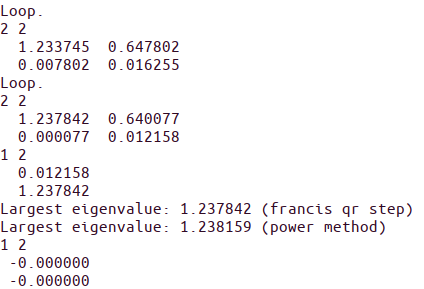
\includegraphics[width=.4\textwidth]{images/eigen-value.png}}
	\label{fig:ex_Vreprest}
	\caption{La plus grande valeur propre retournée(francisQRstep \textit{VS} powerMethod)}
\end{figure}







\section{Implémentation et discussion}


\subsection{Description de l'implémentation}

Prenons $\Ddot{x}=-x$ comme oscillateur harmonique modèle, et qui sera écrit comme deux équations différentielles du premier ordre
  \begin{equation}
    \Dot{x}=p
  \end{equation}

\begin{equation}
    \Dot{p}=-x
\end{equation}

Nous allons intégrer numériquement ces équations par la méthode d'Euler avec conditions initiales ${\left[ 0,1 \right]}^2$ et un pas de temps $h=0,02$ 



La formule pour avancer dans le temps les équations différentielles (41) et (42) sont:
\begin{equation}
   x_{k+1}= x_{k} + hp_{k}   \;\;\;\;\; \;\;   p_{k+1}= p_{k} - hx_{k} 
\end{equation}

On peut écrire la formule utilisée dans ce document pour avancer d'un pas dans la notation matricielle comme
 \begin{equation}
   \left(
  \begin{array}{rrrrrrr}
     x_{k+1}    \\ 
       P_{k+1} \\ 
    
    \end{array}
    \right) =\left(
    \begin{array}{rrrrrrr}
      c & d    \\ 
      -d & c   \\ 
    
      \end{array}
       \right) \;\left(
    \begin{array}{rrrrrrr}
      x_{k}   \\ 
      p_{k}   \\ 
    
      \end{array}
       \right)
\end{equation}

où c et d sont des constantes différentes pour les différents schémas numériques, pour $h \rightarrow{0}$,  $c \rightarrow{1}$ et $d \rightarrow{h}$



\subsection{Discussion}
  Dans cet exemple deux propriétés sont intéressantes à vérifier:
  \begin{itemize}
      \itemperso{} les valeurs de sorties sont inférieures à 1?
      \itemperso{} sont elle bornées ?
  \end{itemize}
  
  
  
  
\subsection{Résultats}


\begin{itemize}
    \itemperso{Recherche de la valeur $Max$ de $x_{k}$} 
    
    prenons $Q= \begin{pmatrix} 
  1 & 0 \\
   0 & 0 
\end{pmatrix}$ et pour un vecteur 
 $\begin{pmatrix} 
  1 \\
   1  
\end{pmatrix}$, la valeur de $K$ sera égal à 221, $K_{1}$ sera égal à 113 
        
   Le $ Max = 1,219 $ à $k=48$, de ce fait la propriété $x_{k} \leq 1$ n'est pas vérifiée.
    
    
     \itemperso{Recherche de la valeur $Max$ de $v_{k}$}
     
       prenons $Q= \begin{pmatrix} 
  0 & 0 \\
   0 & 1 
\end{pmatrix}$ et pour un vecteur 
 $\begin{pmatrix} 
  1 \\
   1  
\end{pmatrix}$, la valeur de $K$ sera égal à 221, $K_{1}$ sera égal à $185 $ 
        
   Le $ Max = 1 $ à $k=0$.
     
     
      \itemperso{Pour la borne}
      
       prenons $Q= \begin{pmatrix} 
  1 & 0 \\
   0 & 1 
\end{pmatrix}$ et pour un vecteur 
 $\begin{pmatrix} 
  1 \\
   1  
\end{pmatrix}$, la valeur de $K$ sera égal à 132, $K_{1}$ sera égal à 132  
        
   Le $ Max = 1,79 $ à $k=0$.
      
\end{itemize}




















\clearpage
\setcounter{section}{0}
\nnsection{Conclusion générale}

\subParagraphe{Conclusion}
\vskip .4cm

En conclusion, ce travail nous a permis d'avoir une première approche sur les problèmes d'optimisation des systèmes à temps discret.Le code développé propose un certain nombre de fonctionnalités de base utiles mais des points restent encore à étudier.


Ainsi, sur cette version finale, nous avons réussi à obtenir une solution précise avec un nombre fini d'évaluations des problèmes d'optimisations rencontrés, aussi Réussir à calculer les critères d’arrêt global pour les systèmes linéaires stables et les propriétés ellipsoïdales. 

Pour continuer ce projet, il serait aussi intéressant de mener un travail sur plusieurs fronts.Le point important focalise sur une grande classe de systèmes non linéaires qui est les systèmes non linéaires affines d'un côté, et d'essayer d'optimiser les entiers après avoir résoudre un problème de minimisation de l'autre côté.

\subParagraphe{Apport personnel}
\vskip .4cm

Ce stage a été très enrichissant pour moi car il m'a permis de découvrir dans le détail le secteur du mathématique basant sur la vérification de systèmes dynamiques tout en mettant l'accent sur l'optimisation mathématique.Aussi il m'a permis de découvrir concrètement la théorie de Lyapunov, la théorie des matrices ainsi la méthode prometteuse de l'optimisation conique qui est la SDP que j'ai particulièrement apprécié.

Ce stage m'a aussi permis de remémorer la programmation C qui est toujours d'actualité dans la programmation système et la robotique et de découvrir d'autres ressources, aussi d'autre librairies en langage C/C++ après l'avoir manipuler. 

Forte de cette expérience et en réponse à ses enjeux, j'aimerai beaucoup par la suite essayer de m'orienter via un autre projet  stage où j'aurais l'opportunité d'appliquer le peu que j'ai, vers le secteur des systèmes distribués et technologies des réseaux  avec des acteurs de petites tailles, et un important développement d'avenir. 






%----> Bibliographie
\newpage

\setcounter{page}{1}
\renewcommand*{\thepage}{A~\arabic{page}}
\addcontentsline{toc}{section}{Références}
%\addbibresource{bib/all_bibs/biblio}
%\printbibliography
%\bibliographystyle{unsrt}
%\bibliography{bib/all_bibs}
%\nocite{*}
\bibliography{bib/all_bibs} 
\bibliographystyle{unsrt}


%
% 3 - Ajout table des matières et liste des figures ; tables
%     Utilisation des préférence utilisateurs :
%          * \whereTOC -> end
%          * \whereLOF -> end
%          * \whereLOT -> end
%          * \TOCLOFTNumStyle -> via le fichier de conf xxx
%     Un réglage manuel comlémentaire est possible sur les \vfill - \newpage
%

%\setcounter{page}{1}
%\renewcommand*{\thepage}{\Roman{page}}

\makeatletter
\ifnum\pdf@strcmp{\whereTOC}{end}=0
\clearpage
\else\ifnum\pdf@strcmp{\whereLOT}{end}=0
\clearpage
\else\ifnum\pdf@strcmp{\whereLOF}{end}=0
\clearpage
\fi\fi\fi

\renewcommand{\sectionbreak}{}
\includeTOC{end}
\includeLOF{end}
%\includeLOT{end}
%\nnsection{Résumé}


\newpage
\pagestyle{empty}
\begin{titlepage}

\begin{figure}[htbp]
 \hbox{
     
\includegraphics[width=40]{images/2.png}
     \hspace*{12.5cm}
     
\includegraphics[width=40]{images/2.png}
 }
\end{figure}

\vspace {-1.8cm}

\begin{center}
%%%%%% En-tete
{\bf Universit\'{e} de Perpignan Via Domitia \\
	\vspace{0.3cm}
   
Master en Mathématiques , Informatique et Modélisation } \vspace{0.2cm}\\

{\bf {\large  Laboratoire de Math\'{e}matiques et Physique }}\\
 
{\bf   UFR Sciences Exactes et Exp\'{e}rimentales } \\

{ \textbf{D\'{e}partement Math\'{e}matiques – Informatique}}\\ \vspace{0.8cm}
%%%%%%%%%%%%%%%%%%%%%%%%%%%%%%%%%%%%%%%%%%%%%%%%%%%%%%%%%
\thColor{\Huge{\textbf{RAPPORT DE STAGE et MÉMOIRE}} \\ \Large{\textbf{Master II}}} \\\vspace{0.3cm}
\large{\emph{\textbf{Spécialité:} CALCUL HAUTE PERFORMANCE, SIMULATION}}\\ \vspace{0.8cm}
\huge{\textbf{Thème}}\\ %\vspace{0.3cm}
\noindent\rule{\textwidth}{1mm}
\Large{\textbf{Vérification de systèmes dynamiques linéaires par
optimisation quadratique}}
\noindent\rule{\textwidth}{1mm}
\end{center}
\vspace{0.3cm}
%%%%%%%%%%%%%%%%%%%%%%%%%%%%%%%%%%%%%%%%%%%%%%%%%%%%%%%%
\begin{tabular}{ p{9cm}  p{6cm} }
\textbf{Encadré par} & \textbf{Réalisé par} \\
\begin{itemize}
	\item \textsc{Assalé Adjé} 
\end{itemize}
&
\begin{itemize}
	\item \textsc{Ryma Nait Amara} 
	
\end{itemize}
\\
\end{tabular}
\vspace{3.5cm}
\begin{center}
2017/2018
\end{center}

\end{titlepage}

\newpage



%\begin{figure}[ht]
  %\caption{Une figure magnifique}
  %\label{fig:mafig}
%\end{figure}

%\begin{table}[ht]
  %\caption{Un tableau vital pour la suite}
  %\label{tab:vital}
%\end{table}


%%% Local Variables:
%%% mode: latex
%%% TeX-master: "../../Template"
%%% End:

\end{document}


%%% Local Variables:
%%% mode: latex
%%% TeX-master: t
%%% End:








